\documentclass[runningheads,a4paper]{llncs}
\pagestyle{plain}
\usepackage{pifont}
\usepackage{color}
\usepackage{appendix}
\usepackage[spanish]{babel}
\usepackage{latexsym} 
\usepackage{multicol}
\usepackage{theorem}
\usepackage{wrapfig}
\setcounter{secnumdepth}{3}
\usepackage[rflt]{floatflt}
\usepackage[utf8]{inputenc}
\usepackage{graphicx}
\usepackage{inputenc}
\usepackage{float}
\usepackage{pdfcolparallel}
\usepackage[colorlinks=true,linkcolor=black,urlcolor=black, citecolor=black]{hyperref}
\graphicspath{{./img/}}
\usepackage{lscape}
\usepackage{setspace}
\DeclareGraphicsRule{.wmf}{bmp}{}{}

\usepackage{color}
\definecolor{gray97}{gray}{.97}
\definecolor{gray75}{gray}{.75}
\definecolor{gray45}{gray}{.45}

\usepackage{listings}
\lstset{ frame=Ltb,
     framerule=0pt,
     aboveskip=0.5cm,
     framextopmargin=3pt,
     framexbottommargin=3pt,
     framexleftmargin=0.4cm,
     framesep=0pt,
     rulesep=.4pt,
     backgroundcolor=\color{gray97},
     rulesepcolor=\color{black},
     %
     stringstyle=\ttfamily,
     showstringspaces = false,
     basicstyle=\small\ttfamily,
     commentstyle=\color{green},
     keywordstyle=\bfseries,
     %
     numbers=left,
     numbersep=15pt,
     numberstyle=\tiny,
     numberfirstline = false,
     breaklines=true,
   }


\lstnewenvironment{listing}[1][]
   {\lstset{#1}\pagebreak[0]}{\pagebreak[0]}

\lstdefinestyle{C}
   {language=C,
   }

\setlength{\theorempreskipamount}{7mm}
\setlength{\theorempostskipamount}{7mm}
\setlength{\parindent}{4pt}
\theoremstyle{break}
\theorembodyfont{\normalfont}
\theoremheaderfont{\scshape\large}
\newtheorem{ejemplo}{Ejemplo} 
\newtheorem{definicion}{Definición}
{\theoremstyle{plain} \newtheorem{defi}{Definición}}
\usepackage{amssymb}
\newcommand{\R}{\mathbb{R}}
\newcommand{\Z}{\mathbb{Z}}
\newcommand{\Q}{\mathbb{Q}}

\usepackage{array}
\newcolumntype{$}{>{\global\let\currentrowstyle\relax}}
\newcolumntype{^}{>{\currentrowstyle}}
\newcommand{\rowstyle}[1]{\gdef\currentrowstyle{#1}%
  #1\ignorespaces
}

\newcommand{\id}{1\!\!l}
\newcommand{\vn}[1]{\mathbf{#1}}
\newcommand{\Mat}[1]{ {\displaystyle #1 } }
\newcommand{\bc}{ \begin{center} }
\newcommand{\ec}{ \end{center} }
\newcommand{\sen}{ \mbox{sen} }
\newcommand{\MP}[2]{ \begin{minipage}{7.8cm}
#1 \end{minipage}
\hfill \begin{minipage}{7.8cm}
#2 \end{minipage}
}
\newcommand{\benu}{\begin{enumerate}}
\newcommand{\eenu}{\end{enumerate}}
\newcommand{\limite}[3]{\lim_{ #1 \rightarrow #2} #3 }

\usepackage{amssymb}
\setcounter{tocdepth}{3}
\usepackage{graphicx}

\usepackage{url}
\urldef{\mailc}\path|cesar.calatrava.ruiz@gmail.com|
\newcommand{\keywords}[1]{\par\addvspace\baselineskip
\noindent\keywordname\enspace\ignorespaces#1}
%%%----------------------------------------------------------------------

\usepackage{marvosym}
\usepackage{fontspec} 					
\usepackage{xunicode,xltxtra,url,parskip}
\RequirePackage{color}
\usepackage[usenames,dvipsnames]{xcolor}
\usepackage[big]{layaureo}
\usepackage{supertabular}

%Setup hyperref package, and colours for links
\usepackage{hyperref}
\definecolor{linkcolour}{rgb}{0,0.2,0.6}
\hypersetup{colorlinks,breaklinks,urlcolor=linkcolour, linkcolor=linkcolour}


%-------------WATERMARK TEST [**not part of a CV**]---------------
\usepackage[absolute]{textpos}

\setlength{\TPHorizModule}{30mm}
\setlength{\TPVertModule}{\TPHorizModule}
\textblockorigin{2mm}{0.65\paperheight}
\setlength{\parindent}{0pt}


%% -- ACRÓNIMOS Y GLOSARIO -----------------------------------------------------
\usepackage[printonlyused]{acronym}

\renewcommand*{\acsfont}[1]{\textsc{\textscale{.85}{#1}}} % enunciado del acrónimo: OO
\renewcommand*{\acfsfont}[1]{#1}
\renewcommand*{\acffont}[1]{#1}

% imprime: "Object Oriented (OO)"
\newcommand{\acx}[1]{\acused{#1}\acs{#1} %
  \nolinebreak[3] %
  (\acl{#1})}

\newcommand{\Acro}[2]{\acro{#1}{#2}\acused{#1}}
\newcommand{\sigla}[1]{\textsc{\textscale{.85}{#1}}}

%baselinestrech
\renewcommand{\baselinestretch}{1.35}

\begin{document}
%Cambiar Cuadros por Tablas y lista de...

\renewcommand{\listtablename}{Índice de tablas}
\renewcommand{\tablename}{Tabla}

%Cambiar Appendice por Apendices
\renewcommand{\appendixname}{Anexos}
\renewcommand{\appendixtocname}{Anexos}
\renewcommand{\appendixpagename}{Anexos}
\renewcommand{\lstlistingname}{Código}
\renewcommand{\lstlistlistingname}{Índice de códigos}

\mainmatter

\tableofcontents
\newpage
\listoftables
\newpage
\listoffigures
\newpage

\large\textbf{RESUMEN}
\textbf{}\\

\large{
Actualmente la proliferación de los documentos electrónicos en el ámbito empresarial, que tradicionalmente constituían conglomerados de papeles en formato físico, es una realidad. Durante los últimos años se ha experimentado una transformación de este tipo de documentos a un nuevo formato, lo que ha conllevado la búsqueda de una solución para la correcta transformación, gestión y procesamiento de la información presente en dichos documentos.



Sin embargo, los sistemas tradicionales de recuperación y tratamiento de esta información no han sido capaces de cumplir las necesidades crecientes, por ejemplo, las búsquedas. El hecho de realizar una búsqueda en los sistemas tradicionales, significaba tener una gran cantidad  de contenido carente de utilidad para los usuarios. Bajo estas premisas, se pretende realizar un análisis de las herramientas existentes para optimizar cada uno de los procedimientos del tratamiento de esta información.

Para ello, se hará uso de diversas herramientas que implementan técnicas de Soft Computing, con el fin de descubrir el conjunto de herramientas más apropiadas para el procesamiento de documentos en un ámbito puramente empresarial.

\textbf{}\\

\textbf{Palabras Clave:} Sistema de Gestión Documental, Detección de idioma, Segmentación léxica, etiquetado gramatical, clasificación, búsqueda, términos relevantes.
}

\pagebreak

\large\textbf{ABSTRACT}
\textbf{}\\

\large{
The proliferation of electronic documents in business, traditionally constituting a huge amount of printed paper, is a reality nowadays. In recent years there has been a transformation of this kind of document to a new format, which has involved the search for a new way to transform, manage and process the information in these documents properly.

However, traditional systems of recovery and processing of this information have not been able to meet the growing needs, as for example, searches. The fact of searching in the traditional systems meant having a very large quantity of useless content to users. Under these assumptions, it is intended to perform a study of the existing tools in order to optimize all the procedures for processing this information.



To do this, we will make use of various tools implementing Soft Computing techniques, in order to discover the most appropriate set of document processing tools in a  purely business context. 

\textbf{}\\

\keywords{Document Management System, Language Identification, Tokenization, Part of Speech Tagging, Classification, Search, Top Terms}
}



\newpage
\section{Introducción}

Cuando se habla de documentos de negocio es inevitable asociar el concepto, con todos los documentos generados a partir de una operación comercial, teniendo ésta un carácter directo o indirecto. Por otra parte también se relaciona con toda aquella documentación producida en la gestión de los procesos empresariales. Estos documentos, pueden ser de tipo contable (como las facturas, billetes de transporte,..), complejos acuerdos legales, cartas circulares, informes estadísticos, etc. Todos ellos, son utilizados a diario en el ámbito empresarial por multitud de personas: analistas de datos, gestores, etc.

Entendiendo a la empresa como una entidad, la utilización de la documentación es una herramienta esencial en el desarrollo de los procesos de la misma, desde varios puntos de vista~\cite{intro:2}. Por ejemplo desde la comunicación o transacciones comerciales, hasta el análisis de productividad o incluso, informes de gastos y beneficios.

El volumen documental que puede ser manejado en las empresas de hoy en día, aumenta de manera exponencial y a una velocidad constante. El almacenamiento de una cantidad ingente de documentos, así como su gestión, se ha convertido en un gran reto para estas organizaciones.

En consecuencia, un buen procesamiento de los documentos de negocio para una empresa, aporta múltiples beneficios como son la mejora de la productividad y de la calidad de los procesos que estas llevan a cabo. Si una  empresa, no tiene control sobre sus propios documentos, así como de su contenido, puede incurrir en múltiples errores que le llevarán a disminuir dicha productividad, a una pérdida de beneficios, duplicación de esfuerzos~\cite{intro:2}, etc.

Un Sistema de Gestión Documental (DMS) se puede definir como un sistema informático, que se utiliza para procesar, almacenar, gestionar y  recuperar los distintos documentos electrónicos y su información~\cite{intro:4}.

Siendo conscientes de los retos expuestos en cuanto al manejo de grandes volúmenes de documentos, los sistemas actuales permiten el almacenamiento y consulta de los mismos haciendo uso de tecnologías web. Estos, pueden ser utilizados tanto para la gestión de documentos en formato físico (que son posteriormente transformados a formato electrónico) así como en los procesos de negocio~\cite{intro:5}.

Por ejemplo, un sistema integral de gestión documental se implementa en~\cite{intro:6}. El sistema propuesto está orientado en gran parte a modelar la gestión de procesos de negocio y en un menor grado a una recuperación simple de información. En este tipo de publicaciones, se exponen gran parte de los problemas que tienen las empresas y que llevan consigo grandes problemas en la gestión y funcionamiento de todos aquellos procesos que realizan.

Algunas causas importantes del problema de la recuperación de información en los documentos empresariales son los procesos automáticos de comprensión de la información y el tratamiento el contenido de los documentos. Debido a ello, cuando se pretende acceder a una información determinada, el resultado frecuentemente es, una gran cantidad de documentos que el usuario no ha solicitado o bien, documentos que si bien encajan parcialmente, no son los deseados.

Con el fin de resolver este problema, en~\cite{intro:8} se propone el uso de un mecanismo para utilizar búsquedas basadas en la información solicitada por el usuario, de la manera más descriptiva posible. Actualmente las posibilidades tecnológicas permiten a los sistemas de gestión de este tipo analizar los textos, hacen uso de algunos \textit{Frameworks} destinados al procesamiento de lenguaje natural no estructurado, como pueden ser “Unstructured Information Management Applications” (UIMA)~\footnote{https://uima.apache.org/ -- Ultima el 8 de Septiembre de 2015} y General Architecture for Text Engineering (GATE)~\footnote{https://gate.ac.uk/ -- Última visita el 8 de Septiembre de 2015}.

El estudio expuesto en~\cite{intro:9}, se fija como objetivo  identificar y registrar aquellas partes estructuradas de un conjunto de documentos, haciendo uso de UIMA. Por otro lado, en otros trabajos previos como~\cite{icai:2014} se pretende optimizar los procesos de recuperación de información para empresas que disponen de un alto número de documentos, haciendo un uso de un DMS.

En este trabajo, el objetivo principal será, el análisis de diferentes herramientas existentes destinadas a cumplir con cada una de las necesidades demandadas por los procesos de recuperación de información, así como, suplir todas aquellas desventajas o carencias de dichos mecanismos, haciendo especialmente hincapié en el rendimiento y la efectividad de las herramientas que forman parte del sistema. Para la consecución de dicho objetivo el estudio se basará en una serie de experimentos que pretender dar con la herramienta/s a utilizar en cada uno de los procesos.

En cuanto a la organización del trabajo, se plantea de la siguiente forma:

En una primera instancia, se realizará una recopilación de toda aquella bibliografía relacionada con el presente estudio, para tratar de analizar las soluciones aportadas por otras empresas u organizaciones en el contexto de trabajo especificado. Adicionalmente, se analizarán las publicaciones científicas más recientes que representen las últimas tendencias en el procesamiento y gestión de documentos de texto de negocio.

Posteriormente se propondrá la construcción del sistema. Se analizará  el flujo de trabajo, así como, las herramientas candidatas a ser evaluadas. Se realizará también una primera aproximación a las pruebas a realizar para buscar una solución optimizada para el sistema.

Tras la realización de los experimentos descritos, se expondrán las conclusiones derivadas de ellos y se elegirá las herramientas más eficientes, de cara a ser integradas en el sistema propuesto.

Finalmente se realizará un resumen a posteriori, que permita dar una visión global al lector acerca de lo que se ha realizado y las conclusiones que se han obtenido. Por otra parte se propondrán ciertas mejoras a realizar en un futuro.

\section{Antecedentes}

En esta sección, se pretender dar una visión general sobre el estado de la cuestión. Primeramente se realiza una breve introducción, describiendo qué es y de qué está formado un Sistema de Gestión Documental, así como, su funcionamiento  y organización básica.

A continuación, se realizará un estudio lo más detallado posible sobre el estado de la cuestión. Ciertas técnicas y procesos llevados a cabo durante procesamiento de lenguaje natural, serán analizadas así como, se estudiará el estado actual y de las mismas, así como, los cambios más recientes, tendencias, aplicaciones, etc.


\subsection{Sistemas de Gestión Documental (DMS)}

Los documentos han constituido en gran parte, la consecuencia de una evolución y transformación de la sociedad. Esta siempre ha requerido plasmar en papel todo aquel contenido que le ha despertado interés y que ha necesitado guardar en un momento dado. Con el paso del tiempo los documentos se han ido transformando a un formato electrónico con la proliferación de los sistemas informáticos, y hoy en día, prácticamente todos se generan, almacenan y tratan en un entorno electrónico.

Los sistemas de Gestión Documental proporcionan un marco de actuación para el trabajo con grandes volúmenes de documentos. Un tipo de Sistema de Gestión clásico puede consistir en un simple explorador de archivos, que hoy en día se encuentran en casi cualquier sistema informático. Sin embargo, en sistemas de gestión documental es algo más. Este debe ofrecer algo más que almacenar y clasificar de documentos.

En este sentido, los DMS pretenden dar toda la prioridad a extraer, recuperar, relacionar y dotar de contexto a un conjunto de documentos. De esta manera, se pretende entre otras cosas, tanto un acceso eficiente a grandes volúmenes de datos como proporcionar mecanismos de recuperación e indexación.


\subsubsection{Aspectos de diseño}
\textbf{}

Todo DMS debe controlar ciertos aspectos en su proceso de diseño~\footnote{ \href{http://www.statetechmagazine.com/sites/default/files/the-principles-of-document-management.pdf}{The Principles of Document Management} }~\footnote{\href{http://samples.sainsburysebooks.co.uk/9781743046593_sample_143621.pdf}{DMS}}:

\begin{itemize}
  \item \textbf{Reproducción}: En esta etapa, se pretende diseñar el sistema a bajo nivel  pensando en él como una de caja negra, de tal manera que se establezca una forma de proporcionar los documentos al sistema y una forma de obtenerlos. 
  
  Una de las preguntas más acertadas para aclarar este aspecto es: ¿Es escaneado un documento vía OCR, tratado y almacenado posteriormente?, ¿Como será mostrado posteriormente al usuario?, ¿Que planteamiento o procedimientos se seguirán para llevar a cabo una extracción y presentación de la información al usuario?
  
  \item \textbf{Publicación}: Todo lo relacionado con el formato y procedimiento de salida de los documentos del sistema debería estar considerado en el diseño de un sistema de gestión documental. Por ejemplo, cómo se van a proveer los documentos, como se van a suministrar al usuario, al sistema, a la web, ...
  
  \item \textbf{Autenticación}: A la hora de diseñar un DMS, también se debe seguir una política acorde a la normativa vigente de cara a la validación del sistema.

  \item \textbf{Validación}: Se refiere a los requisitos que deben cumplir los documentos para realizar un tratamiento eficiente y poder establecer unos límites para acotar el flujo de entrada de documentos y reducir el número de fallos.

  \item \textbf{Integración}: Un aspecto muy importante a abordar para un DMS es el de la integración del sistema en un entorno empresarial. Es decir, como se va a entregar el sistema al cliente y cómo va a diseñarse para adaptarse a sus procesos y sistemas lo más rápidamente posible.

  \item \textbf{Distribución}: Evalúa aspectos más cercanos a la distribución y propagación de los documentos al cliente, en un aspecto más arquitectural.

  \item \textbf{Seguridad y Custodia}: Otro de los elementos más delicados es el establecimiento de una política de seguridad para dichos documentos (qué pasa si existe una pérdida de información, etc..). Y la determinación de un protocolo en cuanto al almacenamiento de los documentos (duración, lugar, ..)

  \item \textbf{Versionado}: Un DMS no solamente debería almacenar los datos o documentos más actualizados, si no que, tiene que establecer un sistema organizativo para el control de la información y/o documentación de manera versionada.

  \item \textbf{Captura de documentos}: La captura de los documentos es otro tema a tratar. Mediante la definición de esta fase, se consigue establecer el tipo de procesamiento de los  ficheros y la manera en que serán introducidos en el sistema.

  \item \textbf{Indexado}: Una vez procesado el contenido de un documento y extraídas todas aquellas informaciones y/o datos que requieren ser guardados para su posterior consulta, el proceso de indexación crea una red de información formada por una asociación entre un identificador y contenido (clave-valor), que permitirá un almacenamiento y consulta más eficiente. 
  En cuanto al rendimiento del sistema de cara al usuario las decisiones tomadas en esta fase suelen ser determinantes en el resultado final del sistema.

  \item \textbf{Recuperación}: Quizás la parte más crítica para un usuario final sea, ¿cómo extraer información de un sistema?. Bien, pues cuestiones derivadas de ésta como son la manera del usuario final de consultar información, cuánto tiempo es requerido para encontrarla, qué fiabilidad da el sistema a la información mostrada, etc. son la punta de lanza del sistema, debido a que constituyen el resultado de todo el trabajo que es realizado internamente.

  \item \textbf{Almacenamiento}: El gran volumen de documentos que termina manejando un sistema de este tipo puede ser inmanejable si se opta por un sistema de almacenamiento de información y documentos ineficiente. Por tanto, es decisivo la elección de un buen mecanismo, herramienta y soporte del almacenamiento.
  
  \item \textbf{Flujo de trabajo}: Este es otro punto crítico del diseño de un Sistema de Gestión Documental, en el cual se decide cómo serán los procesos internos, externos y el flujo de trabajo del sistema desde que entra un documento en el mismo hasta que un usuario final requiere una información contenida en él. A continuación se puede observar un esquema global de lo que sería un flujo de trabajo estándar en un sistema de gestión documental:

\begin{figure}
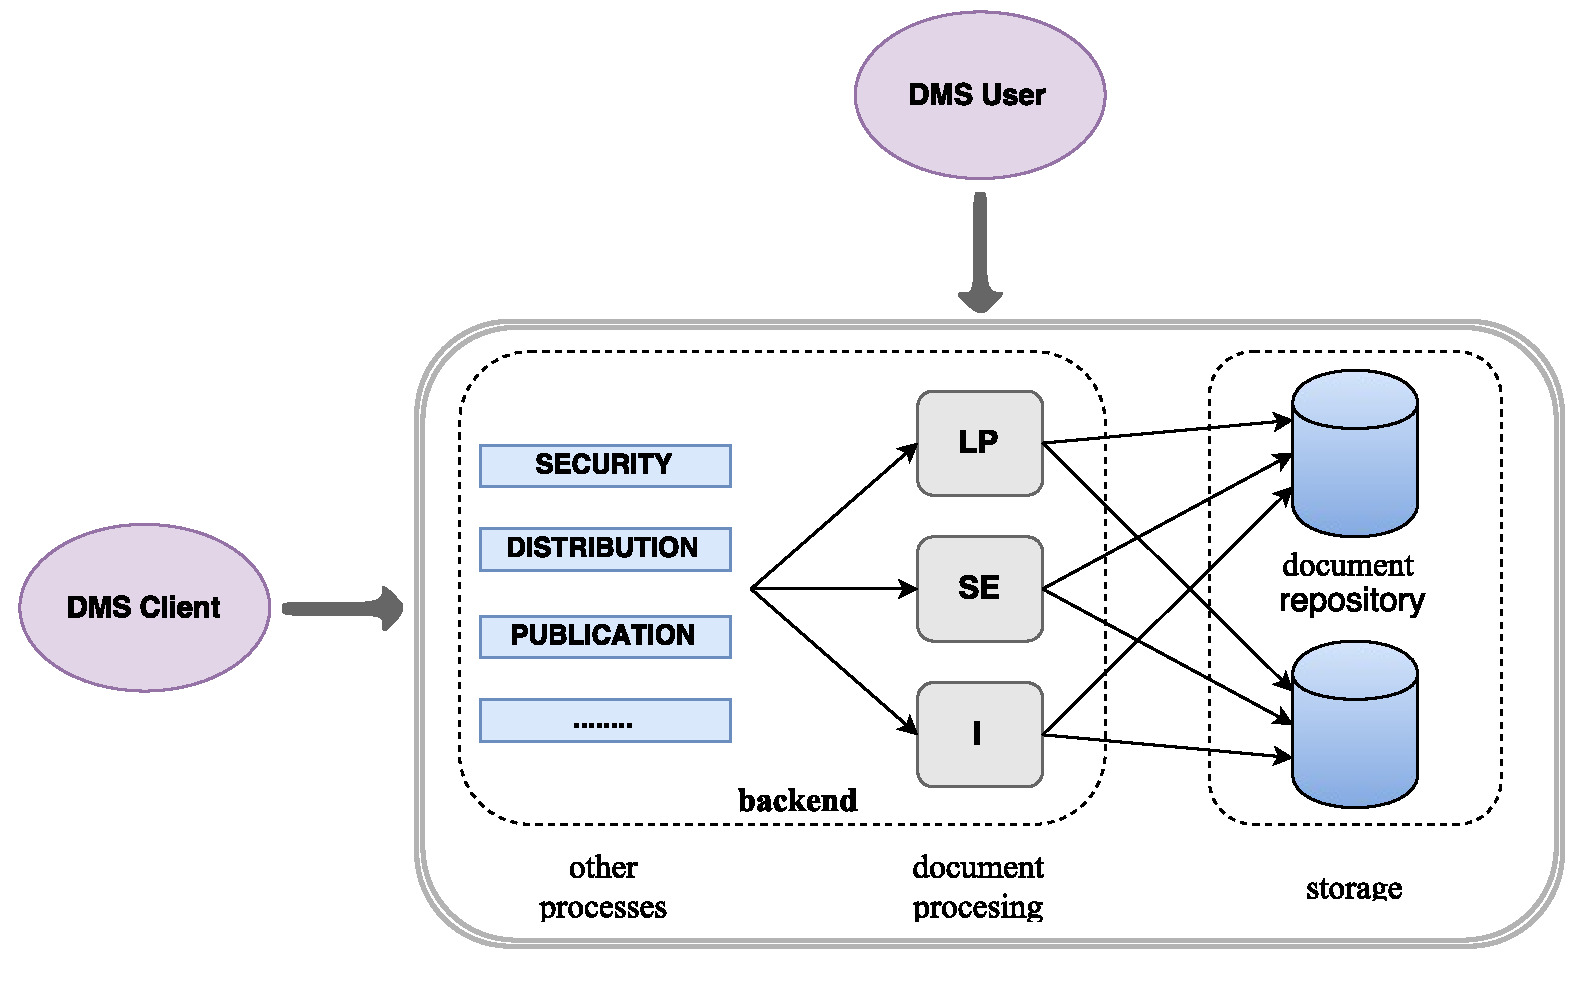
\includegraphics[scale=0.5]{img/standar_workflow.pdf}
\caption[Workflow básico de un DMS]{Workflow básico de un DMS}
\label{fig:standar_workflow}
\end{figure}

  Como se puede observar en la imagen existen dos tipos de usuarios: clientes y usuarios gestores. Ambos accederán a las funciones del DMS haciendo uso de un punto de entrada. Un sistema backend tras esta capa administraría todos aquellos aspectos de infraestructura, seguridad, etc. además de todo los procesos que se apliquen a los documentos. Y finalmente una tercera parte la conformaría el repositorio documental ocupado del almacenamiento.

  \item \textbf{Búsqueda}: La búsqueda de la información, vendría a ser una parte de las políticas establecidas en la Recuperación. Una de las maneras de extraer la información por parte de un usuario, sería el acceso mediante una búsqueda. Estas búsquedas suelen ser presentadas mediante una interfaz sencilla y se suele suministrar a los usuarios de una serie de ``herramientas'' como son sintaxis de búsqueda específica etc., que permitirá una mejora en los resultados extraídos.

  \item \textbf{Clasificación}: Tras la captura, análisis y procesamiento de la información en los documentos, se presenta otra forma de optimización del sistema, que constituye una parte esencial. La clasificación de los documentos es un proceso que, a partir de la información extraída de los documentos, se encarga de agrupar por diferentes propiedades según sea su objetivo o política de clasificación.

\end{itemize}


\subsection{Procesamiento de Lenguaje Natural}

Quizas uno de los legados y bienes mas preciados en la sociedad actual es el conocimiento o información~\cite{nlp:1}. En la era actual, toda esta información es lo que realmente hace que se mueva el mundo, la industria, los negocios, recursos, en fin, se podría decir que la información forma parte muy importante en la vida de los seres humanos.

Desde los primeros tiempos, la información ha sido utilizada, almacenada, gestionada etc, mediante el uso del lenguaje natural, bien sea en un idioma u otro. Como antes se comentaba el gran reto es el almacenamiento y gestión de información y en el, los sistemas informáticos son un elemento esencial. Sin embargo, ellos por sí mismos no tienen la capacidad inherente de entender el lenguaje natural, si no que hay que enseñarles de alguna manera como contextualizarla para convertirla en información útil y caracterizada correctamente.

En este sentido nace un campo de estudio llamado Procesamiento de Lenguaje Natural (PLN o, en inglés, NLP) durante la década de los 60 cuyas raíces principales son la Inteligencia Artificial y la Lingüistica. Su objetivo principal es el estudio y formulación de mecanismos para solucionar los principales problemas derivados de la generación y comprensión de manera automática de los procesos relacionados con el Lenguaje Natural~\cite{nlp:2}~\cite{nlp:3}~\cite{nlp:5}.

Las aplicaciones de la materia~\cite{nlp:4}, pueden ser de distinta naturaleza y van desde la comprensión del propio lenguaje, mejoras en la recuperación de la información hasta búsqueda de respuestas hasta el reconocimiento del habla, síntesis de voz o incluso, traducción automática.

Siguiendo una línea de trabajo encuadrada en este área, la intención es la de evaluar todos todos los procesos posibles que permitan una mejora significativa en el sistema global y que permitan, la contextualización de la información que ellos mismos procesan.

\subsubsection{Detección del idioma}
\textbf{}

Se trata de un proceso que mediante la aplicación de una serie de técnicas y procedimientos, se pretende detectar el idioma sobre el que se recibe una entrada (bien sea vía texto, voz, etc..).

Como bien se expresa en~\cite{lid:1}, el identificador cuasi perfecto idiomático, no deja de ser el ser humano. Con todas las experiencias que este acumula a lo largo de su vida, puede ser identificador de multitud de lenguajes. Gracias a esto, en ocasiones, se identifica una partícula común del lenguaje, en otras, el tono de voz, en otras una pronunciación nasal específica \cite{lid:1}, y en otras simplemente 'Suena como si fuese Portugués'.

De estas experiencias, se puede extraer el conocimiento suficiente para plantear multitud de ideas acerca de la manera más óptima de diseñar una herramienta, que haciendo uso de técnicas de Soft-Computing, permita la identificación de un lenguaje específico. Por ejemplo, por frecuencia de palabras, orden de las letras~\cite{lid:2}, partículas usadas o la identificación de determinadas estructuras únicas de un idioma. Todo ello haciendo uso de un sistema informático va a proporcionar un gran almacenamiento de información y restaría la forma de aplicar una técnica para contextualizarla y conseguir finalmente, dotar al sistema de un protocolo de detección veraz.

Tras la aparente simplicidad de detectar bien o no un idioma, se encuentra un sinfín de aplicaciones muy destacadas, donde el proceso de detección constituye un punto crítico, que es determinante a la hora de realizar un proceso. 
	
\pagebreak
A continuación se enumeran ciertas aplicaciones~\cite{lid:1}:

\begin{itemize}

  \item Por ejemplo es un proceso crítico a la hora de llevar a cabo la gestión de las llamadas para una compañía telefónica en la que intervengan llamadas internacionales, procesos automáticos en los que el interlocutor deba interactuar con una grabación en un determinado idioma.

  \item También relacionada con esta, en los servicios de ayuda a emergencia se pueden dar situaciones ante las cuales una falta de identificación de idioma puede causar incluso la pérdida de bienes materiales o de daños físicos a una persona que necesita ayuda.

  \item En relación a las anteriormente descritas, la compañía telefónica norteamericana llamada AT\&T, provee de un servicio de intérprete para empresas, departamentos públicos y servicios de seguridad en el cual, la identificación del lenguaje es el mecanismo entorno al que giran los demás procesos del servicio.

  \item Agilización en los servicios online de hostelería como paradores, hoteles, etc. en los que una persona puede recibir información y realizar las gestiones en su idioma de manera que automáticamente sea detectado y adaptado el sistema de un idioma a otro.

  \item Sistemas de traducción tanto a nivel escrito como oral. A día de hoy, Google Translate (El servicio de traducción de Google)~\cite{lid:3}, ya dispone de un servicio de identificación del idioma y traducción en tiempo real.
\end{itemize}

En un ámbito puramente científico, se han recuperado multitud de referencias a la detección del idioma. Algunas de estas publicaciones, han sido recogidas en revisiones como la descrita por Pavel Matejka~\cite{lid:4} donde explora los diferentes enfoques en este área hasta el año 2003. Posteriormente existe otra revisión realizada por Roy Pinki et al. \cite{lid:5} que evalúa la documentación más relevante de entre 2003 y 2010. 

Entre 2010 y la actualidad, no se ha encontrado una revisión tan orientada al tema de trabajo presentado en este estudio, sin embargo, se en este rango de años se han desarrollado ciertos artículos que posteriormente serán presentados y que tomarán una gran importancia para la elección final.

\newpage

Durante 2004 se realizaron varios estudios relevantes centrados en el uso de sílabas como unidad mínima en la diferenciación y reconocimiento de un idioma~\cite{lid:6}. Tras este estudio, se comenzó a usar la sílaba como un elemento atómico y mínimo en todo proceso de reconocimiento del idioma. 

Ese mismo año se presenta un estudio muy interesante que pretende analizar todos los métodos probabilísticos propuestos hasta la fecha~\cite{lid:7} para la detección del idioma de un texto (modelo HMM, vectores de frecuencia de trigramas, técnicas de n-gram, ...). El resultado permitió descubrir que la técnica de HMM conseguía una mayor exactitud y velocidad que el resto de métodos durante la clasificación.

Durante el 2006 se realizaron estudios que permitieron evaluar el uso de técnicas como SVM (Support Vector Machine) para la identificación del idioma como~\cite{lid:8} y~\cite{lid:9}, obteniendo una mejora en la identificación y sobre todo en cuanto al rendimiento.

En 2009 se plantea una nueva arquitectura de aprendizaje para la detección del idioma en~\cite{lid:10} y que obtiene como resultado entre un 5-10\% de mejora total sobre la exactitud con la que los sistemas hasta la fecha detectaban un idioma.

En 2012 Marco Lui y Timothy Baldwin de la Universidad de Melbourne, presentan una investigación científica en el área que desarrolla una nueva herramienta llamada ``langid.py''~\cite{lid:11} y que, ayudado de una red bayesiana, varios modelos y una mezcla de la técnica de n-gram consigue un alto rendimiento haciendo uso de multiples corpus y colecciones de datos. 

Adicionalmente es comparada con otras herramientas que a dia de hoy, continuan siendo las mejor valoradas por los usuarios de este tipo de servicios como son: TextCat~\footnote{http://odur.let.rug.nl/vannoord/TextCat/ (Última visita -- 1 de Septiembre de 2015)}, LangDetect~\footnote{http://code.google.com/p/language-detection/ (Última visita -- 1 de Septiembre de 2015)} y CLD~\footnote{http://code.google.com/p/chromium-compact-language-detector/ (Última visita -- 1 de Septiembre de 2015)}. Como se puede observar en su artículo el rendimiento y efectividad es similar con la herramienta LangDetect en ciertos puntos, pero continúa siendo muy superior al de TextCat y CLD.

Este tipo de herramientas ha tenido múltiples usos, siendo el más obvio la detección de idioma de un texto. Por otra parte también se han encontrado ciertos beneficios en el uso del modelo propuesto como en~\cite{lid:12}.

\subsubsection{Segmentación Léxica}
\textbf{}

La segmentación léxica o Tokenization (en inglés), se trata de un proceso mediante el cual se divide una entrada (en este caso texto) en un conjunto de elementos atómicos llamados Tokens. 

Aunque es un proceso muy extendido, no es suficientemente estudiado debido a que se encuentra íntimamente ligado a cada tipo de situación o ámbito de aplicación.

El proceso no debe ser confundido con un mecanismo de limpieza, pues su función no es separar caracteres indeseables, palabras, símbolos o signos. Tampoco el de detectar y suprimir las etiquetas inherentes a un archivo de marcas, ni detectar y eliminar los números de un texto, por no disponer de significado lingüístico. 

La verdadera misión de un Tokenizer es la de separar el texto en unidades atómicas, que pueden ser de distinta naturaleza. Para un ámbito de aplicación el Tokenizer será orientado a la separación de citas, párrafos, palabras, signos o números, tales como son la cantidad de una factura o los beneficios de un informe.

Estudios como el realizado por~\cite{tokenization:1}, tratan de realizar una vista previa de estas técnicas evaluando las alternativas y los últimos avances en la materia. Como conclusión determinan que el proceso de Tokenization es de tipo caja negra debido a su falta de información y convenio entre las funciones de este.

\subsubsection{Etiquetado Gramatical}
\textbf{}

El etiquetado gramatical (Part-of-speech tagging o POS Tagging, en inglés) es es lanzado tras un proceso de Tokenización y su función es la de etiquetar cada uno de los tokens con su clase de palabra. 

Estas clases de palabras van desde nombres, adjetivos, preposiciones, hasta formas verbales. Adicionalmente es capaz de identificar el género de un token y si está en singular o plural.

Esta etapa constituye un punto crítico en el procesamiento de documentos de lenguaje natural dado que es el que tiene un coste mayor  y el que, siendo adecuadamente elegido, puede revolucionar el sistema en cuanto a rendimiento y exactitud. 

\pagebreak

Para elegir un buen etiquetador gramatical, lo primero es entender cómo funciona~\cite{postagger:1}:

\begin{figure}
    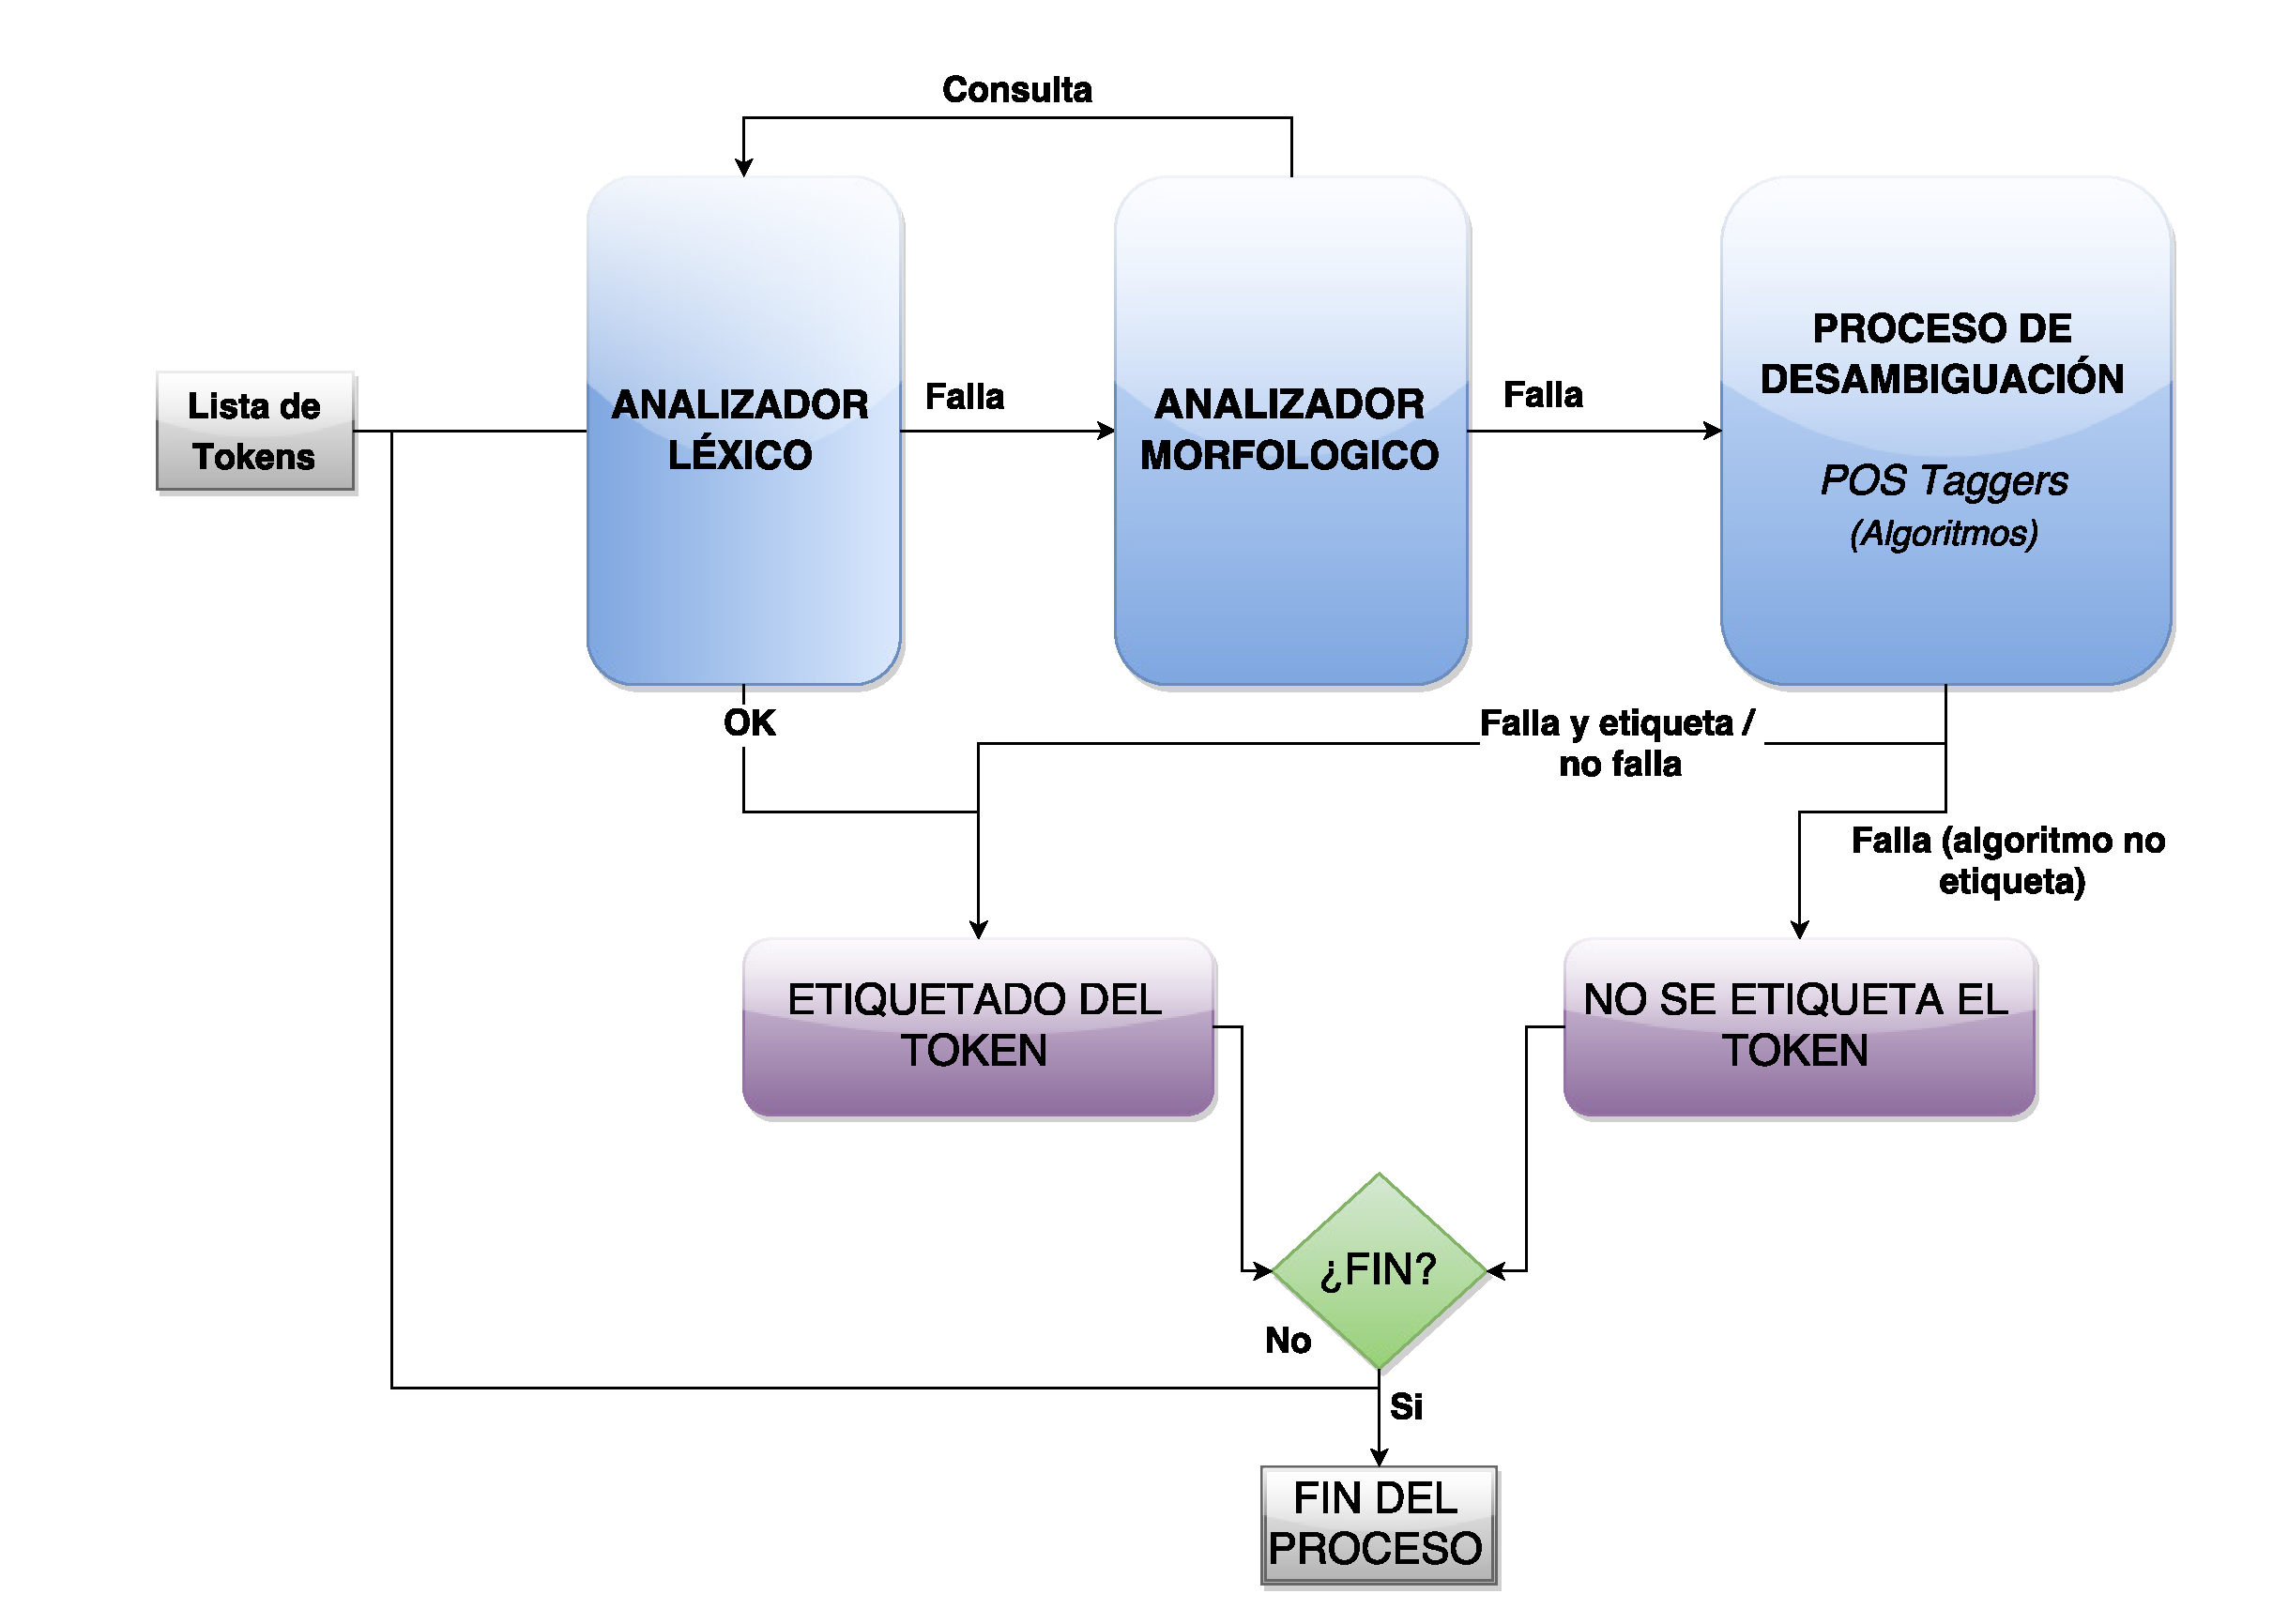
\includegraphics[width=1.0\textwidth]{img/postagger_workflow.pdf}
    \caption[Workflow de un POS Tagger]{Workflow de un POS Tagger}
    \label{fig:postagger_workflow}
\end{figure}

La primera acción tomada por un etiquetador gramatical, es consultar si el token seleccionado se encuentra en un léxico guardado con anterioridad. Si la palabra es identificada se elige la etiqueta correspondiente (en ocasiones hay más de una). En el caso de que esta palabra no se encuentre, continúa mandando el token al analizador morfológico.

El analizador morfológico trata de descomponer dicho token para determinar si contiene un morfema identificable. Una vez hecho esto, manda la palabra descompuesta al analizador léxico una vez más para comprobar si existe. Si lo encuentra, lo etiqueta mediante el proceso antes expuesto, de lo contrario, manda el token al proceso de desambiguación.

En este proceso de desambiguación se aplicarán los diferentes métodos o técnicas de Soft-Computing propuestas. Es la fase que diferencia principalmente un POS tagger y de otro. 

\pagebreak
Por tanto, detectando este como una fase crítica, el objetivo es escoger aquel algoritmo que llegados a este punto, en el que un token no es identificado, ofrezca una mejor relación entre la tasa de éxito y la de rendimiento. 

Cabe destacar un detalle, en el proceso de desambiguación, si finalmente no logra determinar cual es la etiqueta correcta, puede tomar dos vias de trabajo: etiquetar una palabra o bien etiquetarla (sobre todo en modelos probabilísticos) con aquella etiqueta más cercana a él en cuanto a similitud.

Con el objetivo de conocer más acerca de estos mecanismos de desambiguación, a continuación se mostrarán los distintos tipos más relevantes en los que se agrupan, atendiendo a las distintas variaciones:

\begin{itemize}
  \item \textbf{POS Tagger con modelos estocásticos}: Se caracterizan principalmente por hacer uso de un corpus de entrenamiento tales como Brown~\footnote{http://www.hit.uib.no/icame/brown/bcm.html -- Ultima visita 4 de Septiembre de 2015} , Gutenberg ~\footnote{http://www.gutenberg.org/ -- Ultima visita 4 de Septiembre de 2015} o Reuters ~\footnote{http://about.reuters.com/researchandstandards/corpus/ -- Ultima visita 4 de Septiembre de 2015}. Los algoritmos utilizados para este tipo de etiquetador son de tipo probabilístico, de manera que, cada palabra tiene una etiqueta para un contexto dado. Dentro de este tipo de etiquetadores destacan los algoritmos TnT y HunPOS basados obviamente en modelos probabilísticos, más concretamente conocidos como Modelos Ocultos de Markov. El Modelo de Markov (HMM) consiste en descubrir aquellos parámetros desconocidos, a partir de los parámetros observables.

  \item \textbf{POS Tagger basados en reglas}: Los etiquetadores gramaticales basados en reglas son diferentes a los modelos estocásticos. Mientras estos últimos generan una probabilidad para etiquetar ese token y clasificarlo como un tipo de palabra, los basados en reglas, aplican una serie de reglas anteriormente predefinidas para decidir el tipo de token.

  \item \textbf{POS Tagger basados en Transformación}: Combina los dos anteriores. Hace uso de la desambiguación, pero no utiliza reglas previamente definidas, si no que se inducen de forma automática a partir de un corpus de entrenamiento previamente etiquetado. Este algoritmo de inducción es llamado normalmente Brill Tagger~\cite{postagger:2}. Este se define como un tagger destinado al aprendizaje automático basado en transformaciones y dirigido por el error. Consiste en varias fases~\cite{postagger:3} durante las cuales, toma primeramente una muestra de texto no etiquetado y la evalúa en varias fases de etiquetación. Con dicha salida, la compara con el texto correctamente etiquetado y genera una lista de errores cometidos. Para cada error evalúa modificando la plantilla establecida que impacto tiene en cuanto al número de errores de etiquetado globales. Una vez establecido las mejores opciones, se aplica la regla y vuelve a comenzar el proceso, hasta que se sobrepasa inferiormente un umbral de aceptación dado.

\end{itemize}

Todos estos algoritmos son utilizados por las diferentes implementaciones de un POS Tagger concreto, no solo con el objetivo de etiquetar gramaticalmente un texto concreto, si no que son el medio para un fin, es decir, una aplicación que hace un uso indirecto o directo de estas herramientas de procesamiento lingüístico.

El uso más común de aplicación, es el perfeccionamiento de técnicas y/o creación de nuevos tagger basados en algún tipo de algoritmo descrito anteriormente que admita ciertas variaciones o modelos híbridos con el objetivo de tratar con lenguajes algo más complejos como son: el árabe, Malayo, Marathi, Sinhala, Bengalí, Tamil, ... etc.

Sin embargo, las publicaciones recientes, no solo hablan de las maneras de perfeccionar las técnicas que permitan perfeccionar estos procesos, sino en la aplicación de la herramienta en un contexto. Como por ejemplo en un análisis más exhaustivo del procesamiento de mensajes de Twitter (Servicio de Microblogging~\footnote{https://twitter.com/})~\cite{postagger:4}.

También se han realizado estudios en el campo de la Ingeniería del Software, sobre la efectividad de las técnicas de etiquetado gramatical en reportes de bugs~\cite{postagger:5}, con el objetivo de poder preprocesar ese reporte y en un futuro recuperar las palabras claves del mismo.

Por otra parte, el personal sanitario en ocasiones requiere la extracción de los términos más relevantes de un campo o ámbito de estudio dentro de la medicina~\cite{postagger:6}. En este sentido, se desarrolló un trabajo  que procesaba documentación en Español y extraía los términos más relevantes del ámbito de estudio.

Para finalizar cabe destacar el estudio~\cite{postagger:7}, centrado en la traducción automática de documentos de negocio, y donde se analiza detalladamente la construcción de una herramienta POS Tagger orientada a su campo de aplicación.

\subsection{Motores de Búsqueda}

Los motores de búsqueda pueden tener aplicaciones en distintos campos de estudio de la informática. El presente trabajo está centrado en el análisis de las herramientas utilizadas en un sistema de gestión documental, y en este sentido, un motor de búsqueda se refiere al contenido indexado y por tanto se engloba dentro del subcampo de la recuperación de información. En este campo, un motor de búsqueda constituye una herramienta, que haciendo uso de técnicas de búsqueda, permite recuperar documentos o colecciones de documentos indexados en una base de contenidos.

Este tipo de motores de búsqueda, se distinguen de otros como pueden ser los buscadores basados en metadatos o los que contienen la información de cada documento, disgregada en varios campos como puede ser: título, resumen, autor, nombre del fichero, etc.

Cuando se trata de una pequeña cantidad de documentos, el sistema puede permitirse el lujo de realizar operaciones de búsqueda sin tratar de indexar su contenido. Pero cuando en un sistema de este tipo se manejan un volumen elevado de documentos, lo más apropiado es pasar por un proceso de indexación y almacenamiento de la información. Estos procesos se encargan de preprocesar y preparar el contenido para que la recuperación de información realizada por el motor de búsqueda sea lo más eficiente posible.

Los estudios recientes siguen una línea directa de perfeccionamiento de los motores de búsqueda, tal y como se hace en~\cite{contentsearch:1}, o más en el ámbito en el que se desarrolla el proyecto en~\cite{contentsearch:3}.

Por otra parte, se han detectado artículos en los que se desarrollan nuevas arquitecturas y planteamientos para la mejora de los motores de búsqueda, realizando fases de preproceso y evaluación~\cite{contentsearch:4}. Concretamente este último hace uso de las cualidades de Lucene~\footnote{https://lucene.apache.org/ -- (Última visita: 1 Septiembre de 2015)}

Finalmente en cuanto a las propuestas de mejora, hay ciertos artículos como~\cite{contentsearch:2} en los que se centran en la la calidad de los resultados y no tanto en la cantidad, grado de acierto o rendimiento del propio motor. Para ello, proponen un framework destinado a la mejora de la calidad de las búsquedas con el objetivo subyacente de constituir un módulo integrable en los sistemas de búsqueda.

El resto de bibliografía rescatada en la búsqueda actual del tema, se basa en la aplicación y/o modificación de los motores de búsqueda para dotarlos de ciertas características dependiendo del campo de aplicación. Por ejemplo en~\cite{contentsearch:5}, en el que se analiza qué características debería atender un motor de búsqueda en un sistema de gestión de contenido, cuya información pueda ser privada o pública dependiendo del usuario.

\subsection{Extracción de Términos Relevantes}

Los procesos de Extracción de Términos relevantes, como su propio nombre indica, se basan en el análisis de una entrada (en este caso, documentos de texto no estructurado) en el que, siguiendo una serie de métodos y procedimientos, se obtenga aquellas palabras clave que puedan caracterizar dicho documento y diferenciarlo del resto dentro de una colección.

La extracción de Términos relevantes es un proceso ampliamente estudiado y en el que se han dado, evaluado y creado multitud de modelos para la extracción de las palabras claves de un texto. Según Dominich~\cite{topterms:1} los modelos que se pueden seguir en un proceso de recuperación de información son cinco:

\begin{itemize}
	\item \textbf{Modelos clásicos}: modelo booleano, de espacio vectorial y probabilístico.
    \item \textbf{Modelos alternativos}: basados en lógica borrosa.
    \item \textbf{Modelos Lógicos}: basados en la lógica formal.
    \item \textbf{Modelos basados en la interactividad}: ``Incluyen posibilidades de expansión del alcance de la búsqueda y hacen uso de retroalimentación por la relevancia de los documentos recuperados'' \cite{topterms:2}.
    \item \textbf{Modelos basados en la IA}: como por ejemplo redes neuronales, algoritmos genéticos, uso de bases de conocimiento o procesamiento del lenguaje natural.
\end{itemize}

Los modelos más utilizados para la mayoría de las aplicaciones es el de espacio vectorial~\cite{topterms:3} encuadrado dentro de los modelos clásicos, representa un documento como un vector cuyas palabras tienen registrada su frecuencia y haciendo uso de fórmulas muy básicas como la de la frecuencia o la frecuencia inversa, se etiqueta la palabra con un valor cuantitativo en cuanto a su importancia dentro del documento o dentro de la colección.

En el estudio de la bibliografía asociada al proceso, se han encontrado multitud de documentos en los que se proponen variaciones, sobre todo, de los modelos clásicos como el del espacio vectorial, tal que~\cite{topterms:4},~\cite{topterms:5} o ~\cite{topterms:6}.

El resto de aplicaciones que utilizan directa o indirectamente el proceso tienen un amplia gama de campos en los que desarrollar su labor. Estos van desde la extracción de términos relevantes con el objetivo de realizar resúmenes automáticos por ejemplo de una conversación en una red social como se propone en~\cite{topterms:7} hasta la detección de dichas unidades para la recomendación de Tags en Weblogs como se propone en~\cite{topterms:8}.


\subsection{Clasificación de documentos}

La clasificación es el proceso de búsqueda de una serie de modelos o funciones que permiten distinguir entre una serie de clases o conceptos establecidos a priori sobre los datos. Este modelo será utilizado para identificar la clase de los objetos que no han sido clasificados~\cite{han:01}. De esta manera, la clasificación de documentos consiste en asignar una o más clases predefinidas a una serie de documentos de texto tomando como base su contenido~\cite{mer:00}.

En este sentido, el procedimiento de clasificación de documentos, tendría es clave dentro del proceso de distinción de grupos de documentos. Para la consecución de esta etapa del preprocesamiento se harán uso de multitud de técnicas de KDD y Data Mining, concretamente el uso de algoritmos de clustering y de clasificación es cada vez más frecuente en procesos de recuperación de información.

\section{Descripción del Sistema propuesto}
Un Sistema de Gestión Documental suministra las bases para una gestión más eficiente en una organización empresarial mediante la organización e implementación de diferentes herramientas que permitan manejar grandes volúmenes de documentos.

Tras estudiar todos las bases teóricas sobre las que se apoyan los sistemas de este tipo, se propone el diseño de un sistema de gestión documental orientado a un ámbito empresarial, donde se puedan encontrar documentos como pueden ser facturas, albaranes, contratos, etc.

El sistema será descrito en varias pasos. A continuación se describe la composición y flujo de trabajo del sistema propuesto, posteriormente se analizarán todas aquellas herramientas que podrían ser usadas en cada proceso.

El diseño de un sistema de este tipo, como ya se comentó anteriormente, es una labor muy larga y se compone de muchas fases y procesos. Sin embargo, la actual propuesta se centra en el flujo y herramientas relacionadas con los procesos de captura de documentos, preprocesamiento, indexado, almacenamiento, recuperación, búsqueda y clasificación de los documentos que entran en un sistema.

Entrando un poco en detalle, a continuación se muestra un esquema del sistema propuesto. El sistema está compuesto principalmente por dos grandes bloques: un primer componente que se encarga del almacenamiento de los documentos, contenido etc, y un segundo que se encargará de la gestión del sistema de gestión documental y sus procesos subyacentes.

\begin{figure}
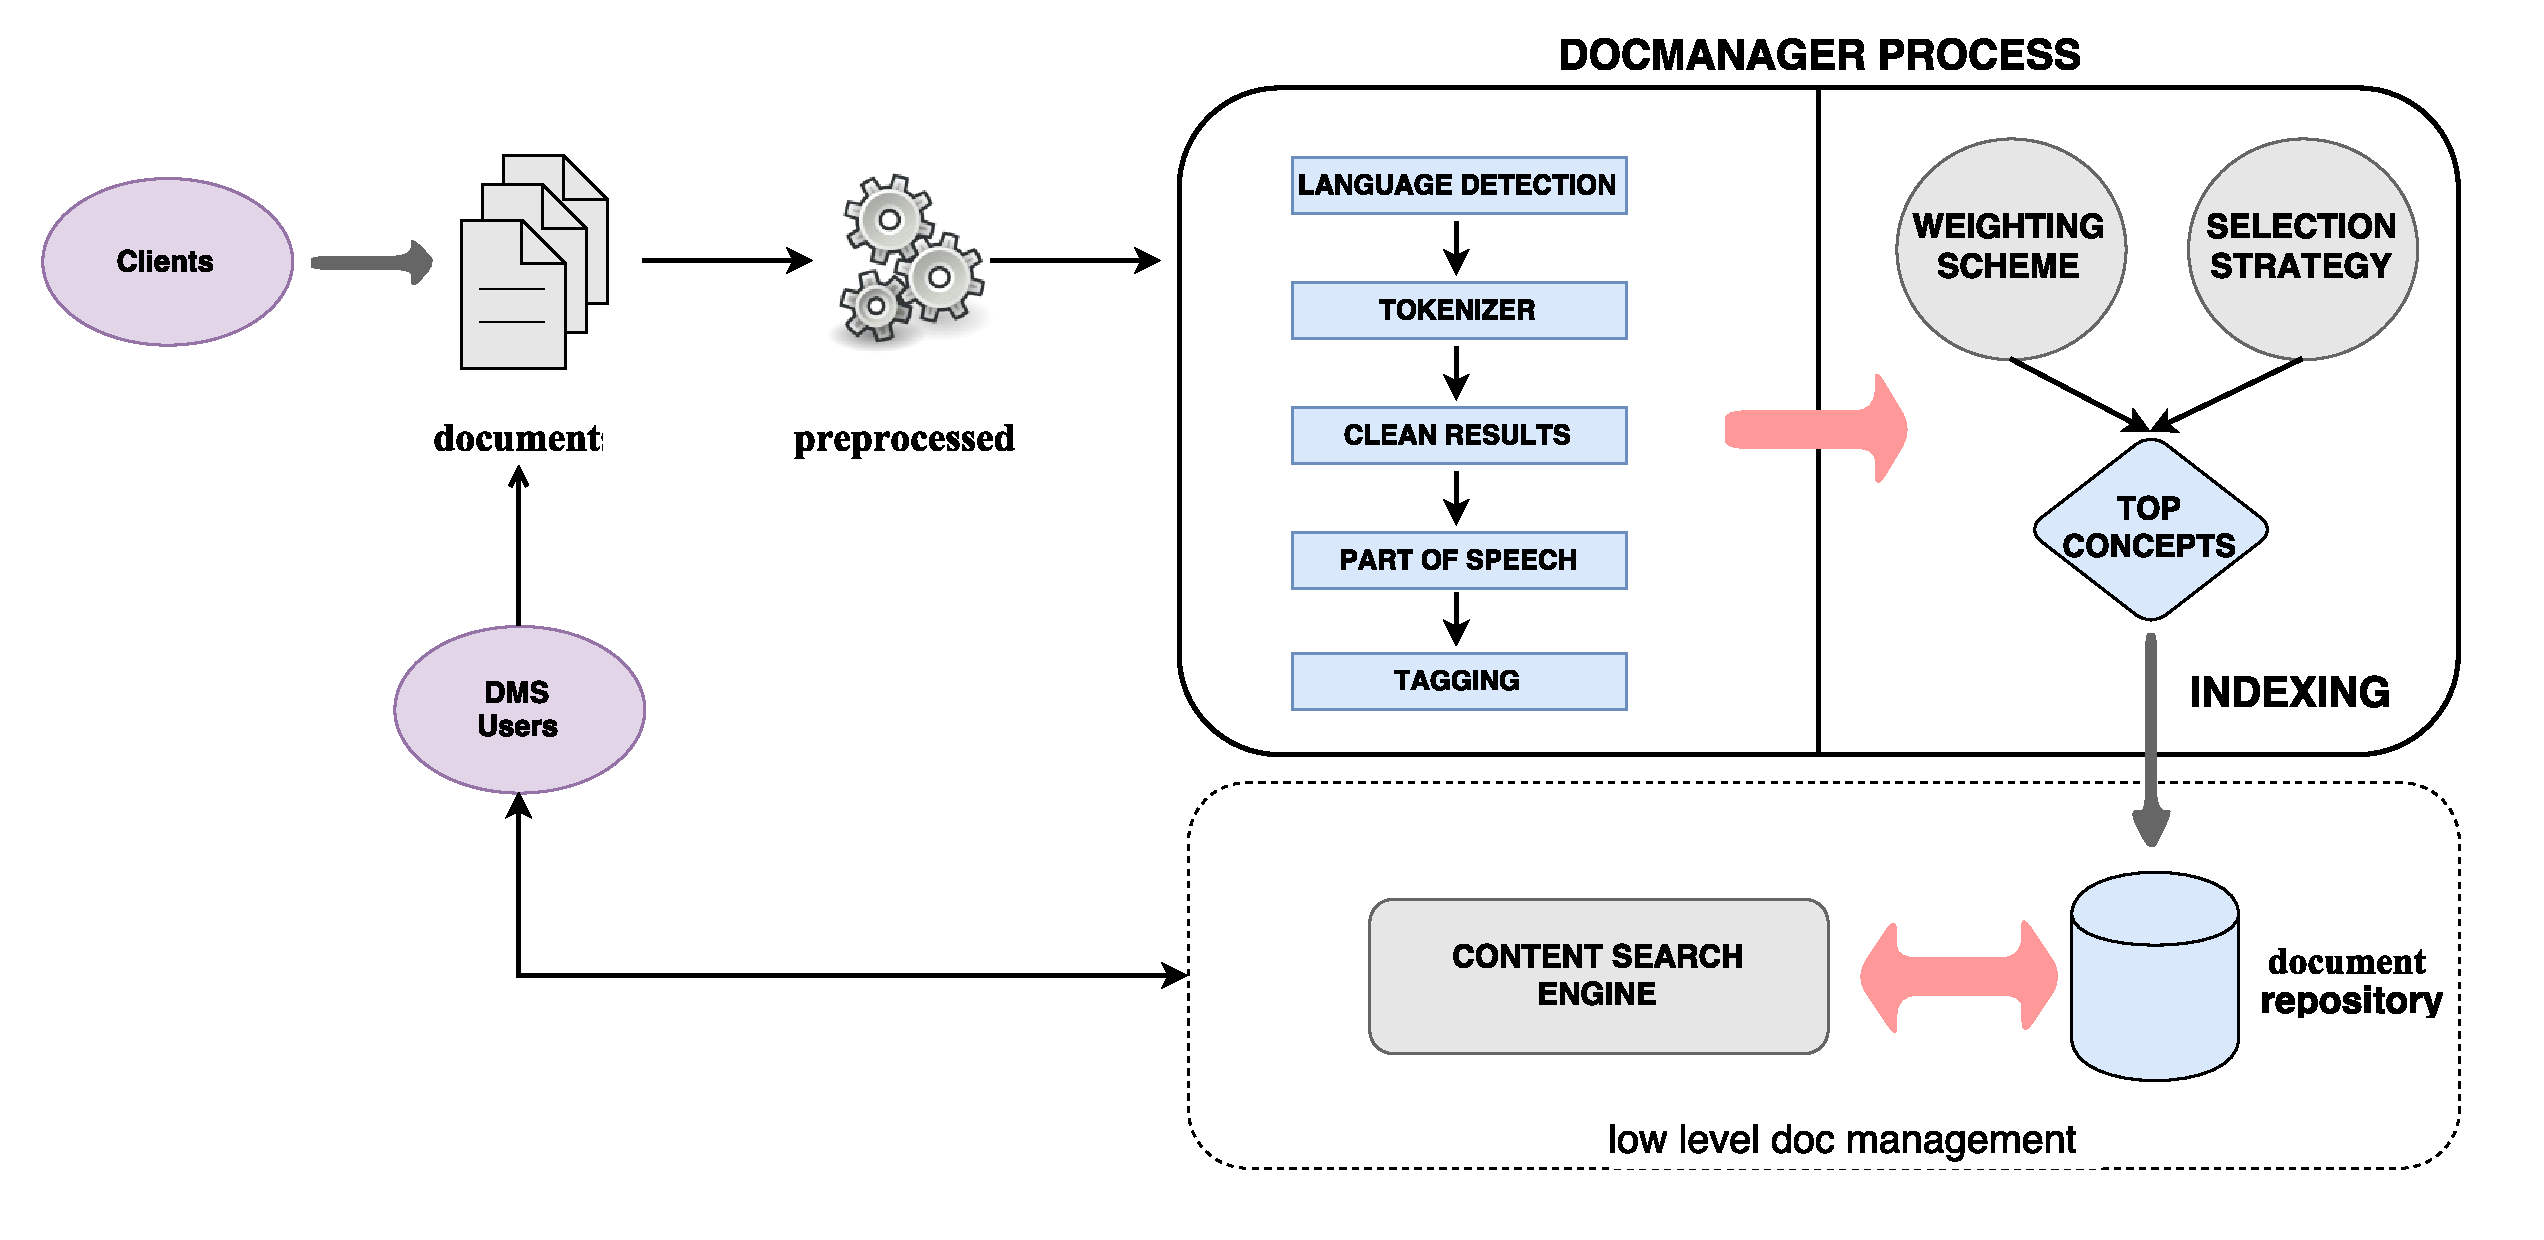
\includegraphics[scale=0.35]{img/propuesta_workflow.pdf}
\caption[Workflow del sistema propuesto]{Workflow del sistema propuesto}
\label{fig:standar_workflow}
\end{figure}

Los usuarios del sistema, pueden hacer uso del mismo via buscador de contenido. Sin embargo también tienen la posibilidad de añadir más documentos al sistema. Una vez que se añade un documento, este pasa por un preproceso, que como puede observarse en la imagen comienza un conjunto de mecanismos de procesamiento de lenguaje natural. 

\pagebreak

Primeramente se evalúa el tipo de documento que es, se transforma en documento de texto plano y se comienza a trabajar con su contenido. Una vez se disponga del contenido se procede a realizar una identificación del lenguaje del documento, ya que sin este, el resto de los procesos pueden  suministrar resultados erróneos. Esto pasa, básicamente porque la mayoría de los algoritmos y librerías disponibles para la realización de estos mecanismos se encuentran bajo un entrenamiento dirigido por un idioma concreto.

El proceso que sigue a continuación es el de segmentación léxica o Tokenizer, mediante el cual se separará el contenido del documento en las mínimas unidades con significado, los tokens. Estos tokens pasarán posteriormente por un proceso de limpieza, en el cual se eliminarán según la política establecida por el sistema y por el tipo de documento, todos aquellos tokens que no serán útiles para un procesamiento lingüístico posterior.

Teniendo un conjunto de tokens con cierta coherencia, se trata de pasarlos por un etiquetador lingüístico para diferenciarlos unos de otros y realizar una selección de aquellos que interesen de acuerdo a la política definida por el sistema.

Una vez seleccionados los tipos de tokens etiquetados que interesen de acuerdo a una estrategia definida son transferidos a un proceso de etiquetado por un valor cuantitativo según su importancia. En este proceso, haciendo uso de técnicas de etiquetado de pesos se extrae un número definido de tokens que constituyen las palabras más importantes y dan todo el significado a un documento y su contenido. Estas palabras, pasan por un mecanismo de indexación que asocia cada una de ellas a un índice determinado y son guardadas en un almacenamiento. Este será usado por un buscador para recuperar la información solicitada.

\section{Experimentación}
Una vez propuesto el sistema, el objetivo es analizar todas aquellas herramientas que puedan permitir dotar al sistema de la máxima efectividad.

\subsection{Medios Utilizados}

Para la realización de las pruebas se ha hecho uso de un ordenador MacBook Pro (2012), con un procesador de 2.3 GHz Intel Core i7, 8GB de RAM DDR3 a 1600 MHz. 

En cuanto a los documentos utilizados para las pruebas, han sido un total de 3 conjuntos de documentos: un primer conjunto correspondiente a 187.073 documentos de actas del parlamento Europeo en 21 idiomas. 

En segundo lugar se ha hecho uso de un set de 1.042.805 documentos empresariales, tales como transacciones bancarias, facturas, etc. extraídos a partir de formularios estándares y datos procedentes de la base de datos de la conferencia de 1999: \textit{``The European Conference on Machine Learning and Principles and Practice of Knowledge Discovery in Databases (ECML PKDD)''}~\footnote{http://sorry.vse.cz/~berka/challenge/pkdd1999/ -- Última visita el 15 de Septiembre de 2015}.

Por último, la empresa DocPath~\footnote{www.docpath.com/ -- Última visita el 15 de Septiembre de 2015} ha cedido un total de 1000 documentos empresariales totalmente anonimizados para llevar a cabo las pruebas. Entre todos hay contratos, facturas, documentos de información interna de una empresa, albaranes, etc. y se pueden encontrar en varios idiomas como Español, Inglés, Catalán, Francés, entre otros.


\subsection{Detección del Idioma}

El primer paso en el procesamiento de lenguaje natural de documentos en el ámbito empresarial, al igual que en otros, es determinar en qué idioma está escrito un documento.

Esta detección debe ser lo más exacta posible, pues la mayoría de las herramientas de extracción de tokens, etiquetado de palabras etc., trabajan en función del idioma, dado que las colecciones de entrenamiento son clasificadas y aplicadas dependiendo del idioma.

En primer lugar, la búsqueda de herramientas de detección de idioma ha llevado a una recopilación de un total de 9. Tras el análisis de sus características, han sido descartadas 5 y las elegidas para su evaluación en el presente estudio han sido las siguientes:
\textbf{}

\begin{itemize}
  \item \textbf{Language-detection}
  \item \textbf{Langid.py}
   \item \textbf{Guess language}
  \item \textbf{LC4J}
\end{itemize}

\newpage

\subsubsection{Language-detection}
\textbf{}

Se trata de una herramienta~\footnote{https://code.google.com/p/language-detection/ - Última visita } open-source, creada por Cybozu Labs, que acredita, un porcentaje de acierto del 99\% de precisión en más de 40 idiomas. En cuanto a su planteamiento interno, la citada herramienta está basada en un filtro Bayesiano que funciona gracias a perfiles creados tras el análisis de resúmenes presentes en la Wikipedia.

\subsubsection{Langid.py}
\textbf{}

Se trata de una herramienta~\footnote{https://github.com/saffsd/langid.py - Última visita} open-source y ha sido creada por Marco Lui de la Universidad de Melbourne y tiene una colección pre-entrenada de perfiles de un total de 97 idiomas. Los datos para su entrenamiento se han extraído de 5 fuentes distintas: JRC-Acquis, ClueWeb 09, Wikipedia, Reuters RCV2, Debian i18n.


\subsubsection{Guess Language}
\textbf{}

La herramienta de Guess Language~\footnote{https://bitbucket.org/spirit/guess\_language - Última visita} fue originariamente desarrollada por Maciej Ceglowski y posteriormente, Jacob R. Rideout la utilizó para desarrollar una nueva herramienta de detección de idioma para KDE. Finalmente Kent Johnson la exportó y mejoró, desarrolandola en Python y actualmente se ha vuelto a actualizar y es mantenida por Phi-Long DO. Se trata de una herramienta basada en la detección de idioma haciendo uso de trigramas y detecta alrededor de 60 lenguajes.

\subsubsection{LC4J}
\textbf{}

Constituye otra herramienta open-source~\footnote{https://github.com/albertjuhe/charikars\_algorithm/tree/master/src/net/olivo/lc4j - Última visita}, destinada a la detección del lenguaje de un documento basada la teoría de N-Grams y descrita en la siguiente~\cite{experiments:1}. La idea tras este planteamiento radica en el uso de TextCat (librería que implementa el algoritmo de categorización). La cantidad total de lenguajes detectados por esta herramienta asciende a los 153 idiomas. 

\subsubsection{Comparativa}
\textbf{}

A continuación se mostrarán los datos estadísticos de cada una de las herramientas con el fin de extraer las conclusiones acerca de su efectividad, rendimiento, etc. Los datos de entrada utilizados, han correspondido a documentos oficiales del Parlamento Europeo, que corresponden a procedimientos, comunicados etc, de hasta 21 idiomas distintos, sumando un total de 187.073 documentos.

\bgroup
\setlength{\tabcolsep}{12pt}
\def\arraystretch{1.5}
\begin{table}
\begin{tabular}{l|c|c|c|c}
\rowstyle{\bfseries}
Herramienta & \rowstyle{\bfseries} Totales & \rowstyle{\bfseries} Detectados & \rowstyle{\bfseries} Precisión & \rowstyle{\bfseries} Tiempo\\ \hline
Guess\_language     & 187073 & 163695 & 87.50\% & 80M 5.83S  \\
Langid.py	        & 187073 & 179885 & 96.15\% & 63M 14.40S\\
Language\_detection & 187073 & 179263 & 95.82\%	& 19M 19.71S\\
Lc4j		        & 187073 & 124918 & 66.77\% & 29M 42.57S\\ \hline
\end{tabular}
\vspace{1em}
\caption{Identificación del idioma: Tabla comparativa de resultados}
\end{table}
\egroup


\vspace{-1.5em}
De la tabla comparativa anterior se puede descartar Guess\_language y Lc4j por un excesivo consumo de tiempo y baja tasa de acierto. Por otra parte los dos candidatos potenciales son Language-detection y Langid.py. Teniendo en cuenta las estadísticas extraídas, la mejor opción es Language-detection.

Si bien es cierto que la precisión de la herramienta Langid.py es ligeramente superior entorno al 0.3\% durante las pruebas llevadas a cabo, hay que tener en cuenta el volumen de documentos analizado y el tiempo que ha llevado.

En ambas herramientas se ha analizado 187.073 documentos en distintos idiomas. Mientras que haciendo uso de la herramienta de Langid.py se ha conseguido una tasa de documentos por segundo equivalente a 49/s, mientras que haciendo uso de language-detection se ha conseguido un total de 161/s. Por tanto ha triplicado el rendimiento por una pérdida del 0.3\% de tasa de efectividad inferior a Langid.py.

Teniendo en cuenta que estas tasas superan el 95\%, se determina que la mejor opción es hacer uso de la herramienta de Language-detection.

\subsection{Segmentación Léxica}

Es el proceso de segmentación de texto en unidades atómicas llamadas tokens. Este, ayudará posteriormente en el tratamiento individual y la determinación de la importancia que tienen estos tokens dentro de un documento o colección.

Una de las partes más importantes en el procesamiento del lenguaje natural tiene que ver con la ruptura de un conjunto de texto en pequeñas unidades que toman el nombre de tokens y que ayudarán posteriormente al procesamiento individual y la determinación de una importancia dentro de un documento o una colección.

En primer lugar se ha llevado un proceso de recopilación de herramientas (librerías, SDK, Frameworks y similares) que permitan el desarrollo de este tipo de operaciones. Tras una primera aproximación se recopilaron un total de 16 candidatos a ser estudiados.

Posteriormente se realizó un estudio individual de cada una de ellas y se descartaron aproximadamente unas 6 debido a su escasa documentación. En una segunda instancia, se re-evaluaron buscando en esta ocasión aquellas herramientas que pudieran encajar de manera más adecuada el ámbito de la gestión documental empresarial. Tras esta evaluación se obtuvieron un total de 5 herramientas para la muestra final de estudio:

\begin{itemize}
    \item \textbf{NLTK Tokenizer}
    \item \textbf{OpenNLP Tokenizer}
    \item \textbf{Mallet Tokenizer}
       \item \textbf{Stanford NLP Tokenizer}
    \item \textbf{Deeplearning4j’s}
\end{itemize}


\subsubsection{NLTK}
\textbf{}

Se trata de una herramienta destinada a suministrar mecanismos para el procesamiento de lenguaje natural. Está compuesta de multitud de librerías y constituye un ``\textit{wrapper}'' de otras lo que hace de esta una herramienta que recopila un gran conjunto de métodos para el procesamiento tanto simbólico como estadístico. Además incluye muestras gráficas así como, corpus preparados, etc. En cuanto al caso de estudio se han seleccionado los siguientes Tokenizer dados por NLTK:

\begin{itemize}
\item \textbf{TreeBankTokenizer}: Usa expresiones regulares para detectar los tokens como en Penn Treebank. La implementación sobre la que se sustentan las pruebas viene dada por Robert McIntyre~\footnote{http://www.cis.upenn.edu/~treebank/tokenizer.sed -- (Ultima visita: 1 de Septiembre 2015}.
\item \textbf{RegexpTokenizer}: Parte el documento usando una expresión regular.
\item \textbf{WhitespaceTokenizer}: Secciona el documento usando espacios.
\item \textbf{WordTokenizer}: Busca, identifica y parte todas las palabras del texto.
\item \textbf{SpaceTokenizer}: Divide el texto por espacios.
\item \textbf{StanfordTokenizer}: Inicialmente diseñado basádose en el PennTreebank 3.
\item \textbf{PunktTokenizer}: Divide el texto en una lista de frases usando un algoritmo no supervisado, previamente entrenado.
\end{itemize}

\subsubsection{OpenNLP}
\textbf{}

Se trata de una API construida en Java y destinada al procesamiento de lenguaje natural, que dispone de multitud de opciones como tokenización, división de documentos por frases, etiquetado de tipo de palabras, parseo de texto, etc. 

El único Tokenizer probado en esta herramienta toma el nombre de “TokenizerME” el cual hace uso de un modelo (\textit{model}) para realizar el proceso de tokenización.

\subsubsection{Mallet}
\textbf{}

Constituye una herramienta desarrollada en Java y destinada al procesamiento de lenguaje natural orientada a una extracción de conclusiones estadísticas, clustering, extracción de información, etc. 

Se ha hecho uso de la clase que contiene destinada a la tokenización de textos llamada StringTokenization y su funcionamiento principal está basado en el uso de expresiones regulares para la separación del texto en tokens.

\subsubsection{DeepLearning4j}
\textbf{}

Se define como un herramienta de \textit{deep-learning} caracterizada por ser de código abierto y distribuida bajo un desarrollo realizado en Java y Scala. Integrado con Hadoop y Spark, DL4J está diseñado para ser usado en un entorno empresarial más que como una herramienta de investigación. Su sección de Tokenizers está compuesta principalmente por 2 ramas:


\begin{itemize}
	\item \textbf{DefaultTokenizer}
    \item \textbf{DefaultStreamTokenizer}
\end{itemize}

\newpage

\subsubsection{Comparativa}
\textbf{}

A continuación se muestran los resultados extraídos de la evaluación de los Tokenizer anteriormente citados haciendo uso del conjunto de documentos empresariales descritos anteriormente:

\bgroup
\setlength{\tabcolsep}{12pt}
\def\arraystretch{1.5}
\begin{table}
\begin{tabular}{p{2cm}|c|p{3.2cm}|c|c}
\rowstyle{\bfseries}
Herramienta & \rowstyle{\bfseries} Herramienta & \rowstyle{\bfseries} Esperados /  \newline Detectados  & \rowstyle{\bfseries} Precisión  & \rowstyle{\bfseries} Tiempo\\ \hline
Default \newline Tokenizer       & deeplearning4j& 23534094 / 16130243 & 68,53\% & 2M 57.15S \\
DefaultStream \newline Tokenizer & deeplearning4j& 23534094 / 20247891 & 86,03\% & 3M 16.03S \\ 
Tokenization            & Mallet        & 23534094 / 23534094 & 100\% & 29M 53.34S \\ 
Tokenizer               & OpenNLP     & 23534094 / 23157829 & 98.40\% & 29M 53.02S \\ 
TreebankWord Tokenizer  & NLTK       & 23534094 / 24564872 & 96.37\% & 8M 14.53S \\ 
Regexp  \newline Tokenizer        & NLTK       & 23534094 / 23534094 & 100\% & 5M 08.23S \\ 
Whitespace  \newline Tokenizer    & NLTK       & 23534094 / 16130243 & 68.53\% & 5M 08.17S \\
word\_tokenize            & NLTK  & 23534094 / 24692577 & 95.90\% & 10M 22.00S \\ 
Space  \newline Tokenizer & NLTK  & 23534094 /  7326205 & 31.13\% & 3M 29.34S \\ 
PunktSentence Tokenizer   & NLTK  & 23534094 /  1170509 & 4.97\% &  4M 27.45S \\ \hline
\end{tabular}
\vspace{1em}
\caption{Segmentación léxica: Tabla comparativa de resultados}
\end{table}
\egroup
\vspace{-1.5em}

Analizando los resultados dados, en un primer análisis es posible el descarted de dos de las herramientas seleccionadas, \textit{SpaceTokenizer} y \textit{PunktSentenceTokenizer},  debido a sus malos resultados en cuanto a precisión. 

También es posible el descarte de \textit{WhiteSpaceTokenizer} de OpenNLP que a pesar de tener una precisión relativamente alta, no puede competir con el resto. 

Una situación similar se puede observar utilizando \textit{DefaultTokenizer} de la herramienta deeplearning4j, pese a su buen tiempo, de algo menos de 3 minutos de procesamiento, su precisión total ha rozado el 69\%. 

\newpage

Tras esta primera selección, las opciones con las que profundizar en el estudio son las siguientes: 

\begin{itemize}
  \item \textbf{DefaultStream Tokenizer} (deeplearning4J)
  \item \textbf{Tokenization} (Mallet)
  \item \textbf{Tokenizer} (OpenNLP)
  \item \textbf{Treebank Word Tokenizer} (NLTK)
  \item \textbf{Regexp Tokenizer} (NLTK)
  \item \textbf{Word Tokenizer} (NLTK)
\end{itemize}

Una vez descartadas las herramientas menos eficientes es necesario establecer claramente la política del sistema de estudio. Debido a que el propósito del presente documento es la mejora de un sistema de gestión de documentos empresariales el análisis de los resultados puede orientarse de múltiples formas: precisión, rendimiento, etc.

Por ejemplo, si el proceso en el que se realiza la segmentación léxica no se realiza on-line (procesos nocturnos, no se garantiza en tiempo real, etc.) y la precisión es una máxima, sin duda, la elección es ``Tokenization'' de Mallet por tener una alta precisión aunque sea peor en cuanto a tiempo gastado en realizar las operaciones.

Si por el contrario se pretende tener una solución más rápida que precisa, se elegiría una herramienta como la de ``WhiteSpace Tokenizer'' de NLTK. Obviamente para una empresa, el objetivo no es hacer las cosas mal y rápido, por tanto, ha sido descartada anteriormente.

Por otra parte, puesto que el presente documento pretende analizar las herramientas más \textbf{eficientes} para cada uno de los procesos dados en estos sistemas, la decisión final será basada en la herramienta que consiga más aciertos en menos tiempo.

Debido a la dificultad para comparar los resultados de las anteriores herramientas, se propone la utilización de una fórmula correspondiente al ratio de la precisión / tiempo:

\[\large R = \frac{\alpha}{\beta }\]

Teniendo en cuenta que $\alpha$ es la precisión y $\beta$ es el tiempo empleado en llevar a cabo el experimento, el resultado será un valor cuantitativo que representa el ratio de la herramienta. De esta manera, a mayor tiempo, menor será el ratio, así como, cuanto mayor sea la precisión mayor será el ratio.

A continuación se muestra un resumen del análisis (Tabla~\ref{tab:tok}):
\bgroup
\centering
\setlength{\tabcolsep}{12pt}
\def\arraystretch{1.5}
\begin{table}
\begin{center}
\begin{tabular}{p{5cm}| c |c|c}
\rowstyle{\bfseries}
Herramienta & \rowstyle{\bfseries} Precisión & \rowstyle{\bfseries} Tiempo (s) & \rowstyle{\bfseries} Ratio\\ \hline
Default Stream Tokenizer 	& 86,03\% 	&  196S  & 0,438 \\
Tokenization				& 100,0\%	&  1793S & 0,055 \\
Tokenizer  					& 98,40\%	&  1793S & 0,054 \\
Treebank Word Tokenizer     & 96,37\%   &  494S  & 0,195 \\
Regexp Tokenizer            & 100,0\%   &  308S  & 0,320 \\
Word Tokenizer              & 95,90\%	&  622S  & 0,150 \\ \hline
\end{tabular}
\end{center}
\vspace{1em}
\caption{Segmentación léxica: Tabla comparativa de resultados II \label{tab:tok}}
\end{table}
\egroup
\vspace{-1.5em}

Realizando un análisis de los resultados obtenidos, se puede asegurar que las 3 herramientas más óptimas en orden son: Default Stream Tokenizer, Regexp Tokenizer, Treebank Word Tokenizer.

La primera es claramente la mejor, sin embargo, cabe destacar que el segundo Tokenizer funciona bajo una expresión regular y mirando la tabla puede obtener un buen tiempo, para una cadena específica.

Por tanto la decisión a tomar dependerá del tipo de documento a usar:

\begin{itemize}
	\item Si tenemos claramente identificado el tipo de documento y sabemos cómo queremos analizar su contenido reduciéndolo a una expresión regular, el Regexp Tokenizer de NLTK es la mejor opción en cuanto a fiabilidad y rendimiento.
    \item Si por el contrario, buscamos un Tokenizer de propósito general y desconocemos el contenido, la elección es Default Stream Tokenizer. 
\end{itemize}


\subsection{POSTagging}

Tras un proceso de extracción de Tokens, se plantea la aplicación de una serie de mecanismos que permitan el etiquetado de dichos \textit{tokens} clasificándolos por su morfología. Esto permitirá posteriormente tanto un análisis más detallado de los tokens, como un filtrado por tipo/s.

La selección de una lista de herramientas es llevada a cabo en varias fases. En una primera instancia se realizó una recopilación masiva de herramientas que pudiesen suministrar dicha funcionalidad, llegando a un total de 16 candidatos. 

En una segunda fase se fueron descartando aquellas herramientas que ya no disponían de mantenimiento, no eran open-source, no disponían de documentación ni información, etc., descartando 5 y dejando un total de 11.

Una vez realizado este primer filtro, se analizó a grandes rasgos la documentación de cada una de las herramientas y se descartaron aquellas que no estaban encuadradas dentro del ámbito de trabajo.

Las herramientas descartadas o bien eran demasiado orientadas a un campo de trabajo no asociado al del caso de estudio, o bien, tenían grandes carencias internas que hacían de esa herramienta una mala elección.

Tras este análisis se seleccionaron un total de seis herramientas para un estudio más detallado.

Una vez evaluadas estas seis herramientas, el estudio se redujo a las tres más relevantes debido a que éstas engloban al resto. Por lo tanto, las herramientas candidatas de estudio para la evaluación del etiquetado de tokens finalmente fueron:
\textbf{}\\

\begin{itemize}
  \item \textbf{OpenNLP POSTagger}.
  \item \textbf{NLTK}.
  \item \textbf{LingPipe}.
\end{itemize}

\subsubsection{OpenNLP POSTagger}
\textbf{}

Esta herramienta utiliza un modelo probabilístico para predecir la etiqueta que aplicar de un conjunto predefinido de las mismas. Por defecto, existen varios modelos para la herramienta que son públicos vía web. Además dispone de la posibilidad de construir un modelo propio mediante el entrenamiento de una muestra dada. 

Los modelos utilizados en las pruebas realizadas son: ``perceptron'' y ``maxent'' (basado en la distribución de probabilidad del principio de máximo de entropía).

\newpage

\subsubsection{NLTK}
\textbf{}

Su principal característica reside en implementa no sólo su propio planteamiento acerca del etiquetado de palabras, sino que, sirve de \textit{wrapper} para un gran conjunto de herramientas open-source con la misma finalidad. De esta manera, aglutina una gran cantidad de alternativas a la hora de llevar a cabo este proceso.

En resumen, las pruebas realizadas han hecho uso de los siguientes POSTaggers:

\begin{Parallel}{0.45\textwidth}{0.45\textwidth}
\ParallelLText{
\begin{itemize}
  \item \textbf{Standard POSTagger}
  \item \textbf{Affix Tagger}
  \item \textbf{Default POS Tagger}
  \item \textbf{Classifier Based POSTagger}
  \item \textbf{Unigram Tagger}
\end{itemize}
}
\ParallelRText{
\begin{itemize}
  \item \textbf{Bigram Tagger}
  \item \textbf{Trigram Tagger}
  \item \textbf{Ngram Tagger}
  \item \textbf{Regexp Tagger}
  \item \textbf{Stanford POSTagger}
\end{itemize}
}
\ParallelPar
\end{Parallel}



\subsubsection{LingPipe}
\textbf{}

La herramienta de etiquetado de palabras de LingPipe, hace uso también del etiquetado basado en modelos estadísticos entrenados de un corpus previamente etiquetado. En las pruebas realizadas, el modelo escogido ha sido el de Brown.

\subsubsection{Comparativa}
\textbf{}

A continuación se muestran los resultados obtenidos tras la evaluación de todos los etiquetadores lingüísticos descritos:

\bgroup
\setlength{\tabcolsep}{10pt}
\def\arraystretch{1.5}
\begin{table}
\begin{tabular}{p{4cm}|c|p{2.5cm}|c|c}
\rowstyle{\bfseries} Etiquetador &  \rowstyle{\bfseries} Herramienta & \rowstyle{\bfseries} Obtenido/\newline Esperado & \rowstyle{\bfseries} Precisión & \rowstyle{\bfseries} Tiempo\\ \hline
StandarPOSTagger 			  & NLTK & 157 / 217 & 72.35\% & 341MS \\
AffixPOSTagger 				  & NLTK & 56  / 217 & 25.80\% & 199MS \\
DefaultPOSTagger (Only nouns) & NLTK & 93  / 94  & 98.93\% & 2MS \\
ClassifierBasedPOSTagger 	  & NLTK & 69  / 217 & 31.79\% & 5677MS \\
UnigramTagger                 & NLTK & 61  / 217 & 28.11\% & 574MS \\
BigramTagger backoff = unigramtagger & NLTK & 62 / 217 & 28.57\% & 1938MS \\
TrigramTagger backoff = unigramtagger  & NLTK & 62 / 217 & 28.57\% & 1461MS \\ \hline
\end{tabular}
\textbf{}\\
\caption{Etiquetado Lingüístico: Tabla comparativa de resultados I}
\end{table}
\egroup




\bgroup
\setlength{\tabcolsep}{10pt}
\def\arraystretch{1.5}
\begin{table}
\begin{tabular}{p{4cm}|c|p{2.5cm}|c|c}
\rowstyle{\bfseries} Etiquetador &  \rowstyle{\bfseries} Herramienta & \rowstyle{\bfseries} Obtenido/ \newline Esperado & \rowstyle{\bfseries} Precisión & \rowstyle{\bfseries} Tiempo\\ \hline
Ngram detected backoff = unigramtagger & NLTK & 60 / 217 & 27.64\% & 1651MS \\
RegexpTagger using backoff = DefaultTagger, only 'NN'  & NLTK & 93 / 94 & 98.93\% & 2MS \\
StanfordPOSTagger (english-bidirectional-distsim) using backoff = DefaultTagger, only 'NN': & NLTK & 168 / 217 & 77.41\% & 5592MS \\
HiddenMarkovModel POSTagger          & LingPipe & 169 / 217 & 77.88\% & 511MS \\
OpenNLP POSTagger (POS Maxent)       & OpenNLP  & 151 / 217 & 69.58\% & 1395MS \\
OpenNLP POSTagger (Perceptron Model) & OpenNLP  & 140 / 217 & 64.51\% & 530MS \\ \hline
\end{tabular}
\textbf{}\\
\caption{Etiquetado Lingüístico: Tabla comparativa de resultados II}
\end{table}
\egroup


Tras realizar un estudio inicial de la tabla, se pueden descartar los siguientes seis taggers dado que ninguno de ellos pasa del 30\% de precisión, y el tiempo empleado en etiquetar es excesivamente alto. 

\begin{itemize}
  \item AffixPOSTagger
  \item ClassifierBasedPOSTagger
  \item UnigramTagger
  \item BigramTagger (backoff = unigramtagger)
  \item TrigramTagger (backoff = unigramtagger)
  \item Ngram (backoff = unigramtagger)
\end{itemize}


Por otra parte de los restantes POSTagger, se descartó el StanfordPOSTagger, debido a que en pruebas más intensivas ha demostrado que es extremadamente lento, resultando 5 veces más lento que el resto de los candidatos no descartados. Una vez finalizada la selección se muestran los resultados de los modelos elegidos haciendo uso Los modelos seleccionados serán analizados tal y como se hizo en el caso de los Tokenizer, haciendo uso de la fórmula del ratio. 

\newpage

En la Tabla \ref{tab:post} se muestran los resultados:


\bgroup
\centering
\setlength{\tabcolsep}{12pt}
\def\arraystretch{1.5}
\begin{table}
\begin{tabular}{p{6.6cm}| c |c|c}
\rowstyle{\bfseries}
Herramienta                                            & \rowstyle{\bfseries} Precisión & \rowstyle{\bfseries} Tiempo (s) & \rowstyle{\bfseries} Ratio\\ \hline
HiddenMarkovModel POSTagger              & 77.88\% & 511MS  & 152.40 \\
OpenNLP POSTagger (POS Maxent)           & 69.58\% & 1395MS & 49.87  \\
OpenNLP POSTagger (Perceptron Model)     & 64.51\% & 530MS  & 121.71 \\
StandarPOSTagger 			             & 72.35\% & 341MS  & 212.17 \\ \hline
\end{tabular}
\vspace{1em}
\caption{Etiquetado lingüístico: Tabla comparativa de resultados III \label{tab:post}}
\end{table}
\egroup
\vspace{-1.5em}

En esta primera tabla se han analizado los POSTagger de propósito general, y se puede ver que el mejor es el ``StandarPOSTagger'' de NLTK. Sin embargo,
hay que destacar como segunda opción  el ``HiddenMarkovModel POSTagger'' de LingPipe, puesto que tiene una precisión superior y la diferencia en cuanto a rendimiento no es muy significativa. Por tanto ambas herramientas serían la mejor elección.

A su vez, se realiza una  comparación para aquellos POSTagger que acotan su etiquetado a una expresión regular o tipo de palabra. Esto es así dado que las condiciones no son las mismas que en los POSTagger de propósito general por tanto, no se pueden comparar con estos. La Tabla \ref{tab:pos2} muestra los resultados obtenidos.


\bgroup
\centering
\setlength{\tabcolsep}{12pt}
\def\arraystretch{1.5}
\begin{table}

\begin{tabular}{p{6cm}|c|c|c}
\rowstyle{\bfseries}
Herramienta                                            & \rowstyle{\bfseries} Precisión & \rowstyle{\bfseries} Tiempo (s) & \rowstyle{\bfseries} Ratio\\ \hline
RegexpTagger using backoff = DefaultTagger, only 'NN'  & 98.93\% & 2MS & 49.46 \\
DefaultPOSTagger (Only nouns)                          & 98.93\% & 2MS & 49.46 \\ \hline

\end{tabular}
\vspace{1em}
\caption{Etiquetado lingüístico: Tabla comparativa de resultados IV \label{tab:pos2}}
\end{table}
\egroup
\vspace{-1.5em}\textbf{}

Como se puede observar, los resultados obtenidos para ambas alternativas en cuanto a tiempo son excelentes.  Cabe destacar
que al igual que pasó con las herramientas del Tokenizer, si se sabe que el etiquetador lingüístico solo trabaja con un tipo de palabra o
podemos reducir su etiquetado a un tipo de token mediante el uso de una expresión regular, estos dos etiquetadores, serían los más óptimos.


\subsection{Extracción de términos relevantes}

El proceso de extracción de términos relevantes va a permitir al sistema identificar qué contenido es reseñable dentro de cada uno de los documentos y por tanto, poder localizarlo en base a su contenido de una manera lo más eficiente posible. Por tanto, un estudio de herramientas que permitan identificar estas palabras, constituye un elemento crucial para la recuperación de información.

Las herramientas encontradas cuyo objetivo es la extracción de términos relevantes de un documento de texto, han sido de diversa naturaleza, así como, muy numerosas. 

La mayoría de estas herramientas, utilizan, como medio de representar los contenidos del documento, el modelo clásico espacio vectorial en sus múltiples formas: frecuencia normal, frecuencia inversa, etc. 

Las herramientas escogidas para realizar este estudio son las siguientes: Samuraizer, Scikit-Learn, Maui, TextBlob y Kea5.

\subsubsection{Samuraizer}\footnote{https://github.com/drikerf/samuraizer -- Última visita: 3 Septiembre 2015}
\textbf{}

Es un proyecto abierto, escrito en Python y publicado en Github \footnote{http://www.github.com/ -- Última visita -- 4 de Septiembre de 2015} consistente en un algoritmo que hace uso de una serie de stop words~\footnote{Palabras que carecen de significado lingüístico y son eliminadas antes de realizar un procesamiento de lenguaje natural} y procesos de stemming ~\footnote{Son aquellos procesos que buscan reducir una palabra a su raíz.} con el objetivo de extraer las palabras más relevantes de un texto.

\subsubsection{Scikit-Learn}\footnote{http://scikit-learn.org/stable/ -- Última visita: 3 Septiembre 2015}
\textbf{}

Se trata de un framework de aprendizaje automático desarrollado en Python y de código abierto, que permite multitud de funciones como clasificación, regresión, clustering, preprocesamiento, etc. Entre sus funciones se encuentra la de extracción de las palabras claves de un texto.
\textbf{}\\
\textbf{}\\
\pagebreak

\vspace{-1em}
\subsubsection{Maui}\footnote{https://github.com/zelandiya/maui -- Última visita: 3 Septiembre 2015}
\textbf{}

Maui es un proyecto originado a partir de la tesis doctoral de Alyona Medelyan, investigador del departamento de Computación de la Universidad de Waikato (Nueva Zelanda). Entre sus funciones está la de extracción de términos relevantes de un texto haciendo uso de tesauros, wikipedia, etc.

\vspace{-1em}
\subsubsection{TextBlob}\footnote{http://textblob.readthedocs.org/en/dev/ -- Última visita: 3 Septiembre 2015}
\textbf{}

TextBlob es una librería creada para Python que trata de suministrar multitud de funciones para los diversos procesos de procesamiento de lenguaje natural y entre ellos la detección de los temas claves del texto de un documento.

\vspace{-1em}
\subsubsection{Kea5}\footnote{http://www.nzdl.org/Kea/ -- Última visita: 3 Septiembre 2015}
\textbf{}

Se trata de la quinta versión desarrollada del algoritmo Kea, diseñado para la extracción de palabras y frases claves dentro del texto de un documento. Es un software de código abierto que ha tenido un largo recorrido en su desarrollo.

\vspace{-1em}
\subsubsection{Comparativa}
\textbf{}

Con el fin de realizar la comparación entre estas herramientas, se han escogido 3 tipos de documentos: contratos empresariales, extractos de transacciones bancarias y registros mercantiles. El objetivo es contar con documentos complejos y comprobar que herramienta detecta el mayor número de coincidencias. Cada documento se ha etiquetado con un máximo de 15 términos representativos.

\bgroup
\setlength{\tabcolsep}{12pt}
\def\arraystretch{1.2}
\begin{table}

\begin{center}
\begin{tabular}{p{4cm}| c| c | c }
\rowstyle{\bfseries} Herramienta & \rowstyle{\bfseries}  Aciertos & \rowstyle{\bfseries} Precisión & \rowstyle{\bfseries} Tiempo (s)\\\hline

Samuraizer        & 5/15    & 33\% & 594MS  \\ % &  0.055 \\
TextBlob		  & 6/15    & 40\% & 1909MS \\ % &  0.020 \\
Scikit-Learn	  & 4/15    & 26\% & 350MS  \\% &  0.074 \\ 
Kea5              & 0/15    & 0\%  & 5000MS \\ %& 0 \\                    
Mallet			  & 7/15    & 46\% & 400MS \\ \hline %0.115
\end{tabular}
\end{center}
\vspace{1em}
\caption{Extracción de Términos relevantes: Tabla comparativa de resultados \label{tab:keywords}}
\end{table}
\egroup
\vspace{-1.5em}

Observando la Tabla~\ref{tab:keywords} no cabe la menor duda que la herramienta con un mejor rendimiento y precisión ha sido Mallet.

% TODO Pon un poco más de vidilla a esto, es decir que pongas más resultados y si es posible que no se te parta la tabla
% TODO Podríamos compararlo con nuestra propuesta que hicimos en el proyecto, eso aportaría mucho.

\subsection{Motores de Búsqueda}
Al manejar y procesar un volumen muy alto de documentos, debe existir un mecanismo de recuperación de información, que, aprovechando todos los procesos anteriores, permite poder obtener el contenido que un usuario requiere mediante una búsqueda, de la manera más eficiente.

Motores de búsqueda, en el contexto que se presenta el trabajo actual, son aquellas herramientas que permiten, indexar, buscar, y procesar los documentos de un DMS. Si bien soportan un pequeño pre-procesamiento, no es utilizado y realmente se ha desacoplado dicho pre-procesamiento en los mecanismos anteriores, para obtener un mayor control de los mismos.

El propósito de las pruebas realizadas en este apartado es elegir aquél que sea más óptimo para realizar su trabajo dentro del sistema propuesto teniendo en cuenta parámetros como rendimiento en la  indexación, precisión en las búsquedas, carga del sistema, etc.

En la primera fase de estas pruebas se ha realizado un estudio exploratorio con el fin de  descubrir los motores de búsqueda más utilizados actualmente, otros desconocidos pero muy eficientes, etc..  Como resultado de esta fase se obtuvieron un total de 11 de candidatos de evaluación.

Tras esta selección preliminar, se estudiaron las características básicas de cada uno de los motores de búsqueda seleccionados. Como resultado, se descartaron 7 motores debido a una escasa documentación, motores que dejaron de ofrecer soporte y congelaron el mantenimiento, no se trataban de herramientas con una licencia de código abierto, etc.

Los 4 candidatos restantes, pasaron por un proceso de evaluación más profunda, descartandose dos por tener una arquitectura muy acoplada a una tecnología concreta (sistema operativo, etc.), quedando los siguientes dos candidatos para la evaluación final:
\textbf{}\\

\begin{itemize}
  \item \textbf{Solr}
  \item \textbf{ElasticSearch}
\end{itemize}

\pagebreak

\subsubsection{Apache Solr}
\textbf{}

Se trata de un motor de búsqueda basado en Apache Lucene pero con una gran cantidad de mejoras que permite distinguirlo de Lucene. 

Por tanto aparte de un motor de búsqueda, Solr incorpora nuevas funciones como pre-procesamiento automático, parseo de documentos en todo tipo (Word, PDF, txt...), clustering, soporte para distintas bases de datos, replicación de índices, búsquedas distribuidas, posee una arquitectura que le permite construir sistemas escalables,..


\subsubsection{ElasticSearch}
\textbf{}

Esta herramienta tiene su origen en Compass~\footnote{http://compass-project.org/ -- Ultima visita 5 Septiembre 2015}, la cual a su vez, esta basada en Lucene. Posee una gran versatilidad en cuanto a soluciones de búsqueda y destaca por una gran capacidad de escalabilidad y por ser distribuido.

\subsubsection{Comparativa en cuanto a la Indexación}
\textbf{}

Para esta prueba se ha tratado de indexar 1042805 documentos, sin meter ningún campo extra en Solr (estructura por defecto) y su equivalencia en ElasticSearch, constituida por una estructura básica. A continuación se muestran los resultados

\bgroup
\setlength{\tabcolsep}{10pt}
\def\arraystretch{1.8}
\begin{table}
\begin{center}
\begin{tabular}{p{2.2cm}|c|c}

\rowstyle{\bfseries} Herramienta & \rowstyle{\bfseries} Numero de Documentos & \rowstyle{\bfseries} Tiempo empleado \\ \hline
Solr          & 1042805 & 1H 7M 22.54S \\
ElasticSearch & 1042805 & 2H 17M 54.01S \\ \hline
\end{tabular}
\end{center}
\vspace{1em}
\caption{Indexación: Tabla comparativa de resultados I}
\end{table}
\egroup
\vspace{-1.5em}

Como se puede observar en la tabla, la indexación en Solr ha tardado significativamente menos que la realizada con ElasticSearch. Mientras que en Solr ha llevado una tasa de indexación de 258 documentos por segundo, en ElasticSearch esta tasa ha sido de 126 documentos por segundo.

\subsubsection{Comparativa de eficiencia en Búsquedas}
\textbf{}

En esta sección se comprobará la eficiencia de cada uno de los motores, realizando una serie de búsquedas. Para ello se plantean unas serie de consultas relacionadas con el millón de documentos usado en otras pruebas. A continuación se muestra un cuadro resumen acerca de las consultas y el objetivo de cada una:

\bgroup
\setlength{\tabcolsep}{10pt}
\def\arraystretch{1.8}
\begin{table}
\begin{tabular}{c|p{5cm}|p{5cm}}

\rowstyle{\bfseries} Query id & \rowstyle{\bfseries} Descripción & \rowstyle{\bfseries} Query \\ \hline

1 & Pagos de seguros pero que NO proceden de otros bancos & ``remittance to another bank'' AND ``stands for insurance payment'' \\
2 & Transacciones con balance negativo con sanción en la región de Cesky Krumlov & ``sanction interest if negative balance'' AND ``Cesky Krumlov'' \\
3 & Extracciones de pensiones en la región de Plzen en el banco MN & ``stands for old-age pension'' AND ``Plzen'' AND ``MN'' \\
4 & Ingresos para pago de préstamos en la región de Praga y el banco EF & ``stands for loan payment'' AND ``Praha'' AND ``EF'' \\ \hline
\end{tabular}
\vspace{1em}
\caption{Búsqueda: Consultas a ejecutar}
\end{table}
\egroup
\vspace{-1.5em}

Como se puede observar, las consultas escogidas son un ejemplo perfecto de búsquedas que un usuario normal haría en un sistema de gestión documental. El hecho de consultar pagos de un seguro que cumplan ciertas condiciones o transferencias asociadas a una región geográfica, así como, otras operaciones como ingresos o extracciones realizadas en otros bancos, son a dia de hoy comunes y representan un ejemplo perfecto debido a su carga de significado lingüístico. 

Cabe destacar que las iniciales descritas en las anteriores consultas como lo son ``MN'', ``EF'' representan el nombre del banco, que por razones de anonimato ha sido sustituido por 2 letras en todos los documentos con los que se realizarán las diversas pruebas.

En las Tablas ~\ref{tab:elastic} y~\ref{tab:elastic2} se pueden observar los resultados del estudio comparativo llevado a cabo:

\bgroup
\setlength{\tabcolsep}{10pt}
\def\arraystretch{1.6}
\begin{table}
\begin{tabular}{l|c|c|c|c|c}

\rowstyle{\bfseries} Herramienta & \rowstyle{\bfseries} Query & \rowstyle{\bfseries} Encontradas & \rowstyle{\bfseries} Correctas & \rowstyle{\bfseries} Precisión & \rowstyle{\bfseries} Tiempo\\ \hline

ElasticSearch & 1 & 18340 & 18320 & 99.90\% & 21MS \\
Apache Solr   & 1 & 18342 & 18320 & 99.88\% & 66MS \\ \hline

\end{tabular}
\vspace{1em}
\caption{Búsqueda: Tabla comparativa de resultados I\label{tab:elastic}}
\end{table}
\egroup

\newpage

\bgroup
\setlength{\tabcolsep}{10pt}
\def\arraystretch{1.6}
\begin{table}

\begin{tabular}{l|c|c|c|c|c}

\rowstyle{\bfseries} Herramienta & \rowstyle{\bfseries} Query & \rowstyle{\bfseries} Encontradas & \rowstyle{\bfseries} Correctas & \rowstyle{\bfseries} Precisión & \rowstyle{\bfseries} Tiempo\\ \hline

ElasticSearch & 2 & 31 & 31 & 100.0\%   & 19MS \\
Apache Solr   & 2 & 31 & 31 & 100.0\%   & 16MS \\
ElasticSearch & 3 & 116 & 116 & 100.0\% & 27MS\\
Apache Solr   & 3 & 116 & 116 & 100.0\% & 32MS \\
ElasticSearch & 4 & 99 & 99 & 100.0\% & 18MS\\
Apache Solr   & 4 & 99 & 99 & 100.0\% & 30MS\\ \hline

\end{tabular}
\vspace{1em}
\caption{Búsqueda: Tabla comparativa de resultados II \label{tab:elastic2}}
\end{table}
\egroup
\vspace{-2em}

En las anteriores tablas se hace patente la potencia de ambos motores de búsqueda en cuanto a la recuperación de información. En la primera petición, la precisión de ElasticSearch ha sido ligeramente superior que en Solr, sin embargo, ha tardado 3 veces más en servirla.

Para el resto de peticiones las consultas han sido resueltas con una precisión del 100\% tanto para Solr como para Elasticsearch, siendo este último ligeramente más rápido en encontrar y servir las peticiones del usuario.

Por tanto, se puede determinar que en cuanto a la recuperación de información basada en búsquedas, ambos sistemas dan resultados muy similares, siendo ligeramente superior ElasticSearch.

\vspace{-1em}
\subsubsection{Comparativa en cuanto a pruebas de Carga}
\textbf{}

Las pruebas de carga de los motores de búsqueda, tienen como objetivo observar el comportamiento de estos bajo una situación de gran número de peticiones. 

Evidentemente, si un DMS es implementado en una organización de un considerable tamaño, el tiempo de respuesta y la capacidad del son elementos que condicionan drásticamente su eficiencia debido a su uso constante y continuado.

Para llevar a cabo las pruebas de carga en ElasticSearch y Solr, se ha utilizado la herramienta Gatling\footnote{http://gatling.io/ -- Última visita 29 Agosto de 2015}. Gatling es un framework open-source escrito en Scala y destinado a la realización de pruebas de carga y estrés, orientada en gran medida a la evaluación de peticiones masivas vía HTTP.

Para la realización de las pruebas de carga en ElasticSearch y Solr, se ha utilizado el mismo índice con un millón de documentos ya mencionado en la sección anterior. 

De la misma forma, se ha utilizado la petición de ``\textit{Pagos de seguros pero que NO proceden de otros bancos}'', evaluada en la sección comparativa de búsquedas. Otra de las condiciones para la prueba ha sido el acceso concurrente de 100 usuarios que realizarán de manera simultánea 10.000 peticiones cada uno, es decir, un total de 1 millón de peticiones. En la Tabla~\ref{tab:carga} se muestran los resultados obtenidos:

\bgroup
\setlength{\tabcolsep}{10pt}
\def\arraystretch{1.6}
\begin{table}
\begin{center}
\begin{tabular}{l|c|p{2cm}|c|c|p{2cm}}
\rowstyle{\bfseries} Motor & \rowstyle{\bfseries} Total & \rowstyle{\bfseries} Petición /\newline segundo & \rowstyle{\bfseries} Max & \rowstyle{\bfseries} Media & \rowstyle{\bfseries} Desviación \newline Estándar \\ \hline
ElasticSearch & 1 Millon &  262.190/s & 1026MS & 381ms & 62 \\
Apache Solr   & 1 Millon &  4560.85/s & 203MS & 20ms & 19 \\ \hline

\end{tabular}
\end{center}
\vspace{1em}
\caption{Pruebas de Carga: Tabla comparativa de resultados\label{tab:carga}}
\end{table}
\egroup
\vspace{-1.5em}

Como se puede observar, a pesar de mantener las mismas condiciones para ambas herramientas, el resultado en cuanto a peticiones por segundo es bastante superior en la herramienta SOLR. Otro de los factores más importantes a tener en cuenta es el tiempo máximo de espera. En este caso también Solr ha obtenido la mejor valoración ya que ha sido 5 veces más rápida en sus peticiones más pesadas. Desde otro punto de vista, el tiempo medio de respuesta en Solr ha sido de 20 ms mientras que, en ElasticSearch ha sido de un total de 381ms. 

La desviación estándar es otro parámetro a tener en cuenta, en Solr es prácticamente idéntica a la media, lo que quiere decir que podría darse la situación de que, ante un retraso de la petición, se hubiesen podido ejecutar 2, es decir el 100\%. 

Sin embargo, a pesar de que para ElasticSearch este medida a priori parece peor, al tener una desviación de 1/5 aproximadamente menor, los retrasos en una petición no afectarían tanto. 

Entrando algo más en detalle, en la Figura~\ref{fig:carga_esearch} se puede observar el rendimiento ofrecido por el motor de búsqueda de ElasticSearch, en cuanto a las respuestas proporcionadas por unidad de tiempo. 

De ella cabe destacar la distribución de tiempos por el número de peticiones: el 99\% de las peticiones ha tardado menos de 578ms y el 75\% de las peticiones han tardado menos de 406ms, por último el 50\% del total de las peticiones ha tardado menos de 358ms.

\begin{figure}
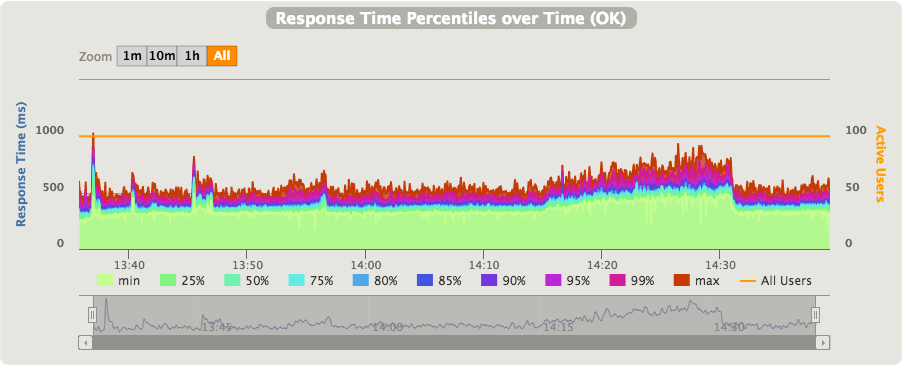
\includegraphics[scale=0.5]{img/es_gatling.png}
\caption[Resumen de los resultados de las pruebas de carga en ElasticSearch]{Resumen de los resultados de las pruebas de carga en ElasticSearch}
\label{fig:carga_esearch}
\end{figure}

Por el contrario, en la Figura \ref{fig:carga_solr} de resultados de Solr, ha mostrado mejoras sustanciales en cuanto a la tasa de peticiones por tiempo. El 99\% de las peticiones ha tardado menos de 71ms, el 75\% menos de 35 y el 50\% menos de 14ms. Cabe destacar que la zonas de color rojo, que se muestran tan agudas, son el resultado de la desviación estándar anteriormente explicada.

\begin{figure}
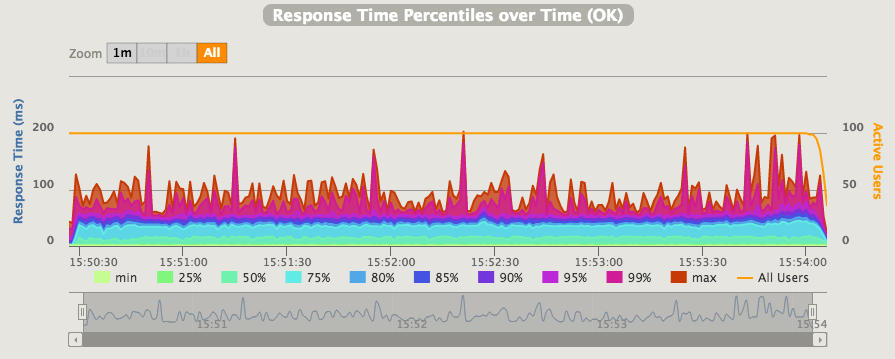
\includegraphics[scale=0.5]{img/solr_gatling.png}
\caption[Resumen de los resultados de las pruebas de carga en Solr]{Resumen de los resultados de las pruebas de carga en Solr}
\label{fig:carga_solr}
\end{figure}

Como se ha podido observar, todos las pruebas indican que la mejor opción para la implementación de un Motor de Búsqueda, dada la infraestructura en la que se han realizado las pruebas, es Solr.


\subsection{Clasificación de Documentos}

Al manejar y pre-procesar un volumen muy alto de documentos, es importante distinguir su tipo y para ello, el proceso de clasificación es crucial. Este proceso va a permitir tener localizados los documentos de negocio de cada tipo de manera que, se pueda utilizar de una manera mas eficiente (pre-procesamiento, búsquedas, etc), sabiendo de qué tipo será el contenido del documento y cómo estará estructurado.

Durante el proceso de búsqueda de una herramienta que cumpla esta función, se han encontrado un gran número de herramientas muy ad hoc a un entorno de aplicación o bien, la mayoría pretendía profundizar en la mejora de los algoritmos de clasificación existentes. Por tanto, la búsqueda como tal de una herramienta que permita la realización de clasificación de documentos textuales de manera genérica, ha conllevado la búsqueda de herramientas realizadas por la comunidades de código libre como Github. Estas herramientas han sido construidas en base a frameworks de procesamiento de lenguaje natural y aprendizaje, en las cuales implementan los algoritmos de clasificación.

Tras una extensa búsqueda, se encontraron un total de 17 herramientas candidatas a ser evaluadas, las cuales posteriormente fueron reduciéndose en 3 etapas. En una primera fase se descartaron todas aquellas herramientas que están altamente ligadas a un problema y que no sería posible utilizar para un propósito general, quedando un total de 10. En una segunda parte, se descartaron aquellas herramientas con poca documentación, que han dejado de dar soporte, etc. hasta obtener un total de 5 candidatas. Finalmente se realizó un estudio más profundo sobre cada herramienta y se descartaron 2 debido a sus características internas (desarrollos incompletos, poco estables, etc). Finalmente se eligieron las siguientes herramientas a ser evaluadas:

\begin{itemize}
	\item Mallet \footnote{http://mallet.cs.umass.edu/ -- Ultima visita el 10 de Septiembre}
    \item Document-Categorization (NLTK + Scikit-Learn\footnote{ http://scikit-learn.org/-- Última visita el 10 de Septiembre.}) \footnote{https://github.com/Ehtaga/document-categorization -- Ultima visita el 10 de Septiembre}
    \item NLTK   \footnote{http://www.nltk.org/book/ch06.html -- Ultima visita el 10 de Septiembre}
\end{itemize}

\subsubsection{Mallet}
\textbf{}

Una de las herramientas ya conocidas y evaluada anteriormente en otros campos del aprendizaje automático, como ha sido en los procesos de segmentación léxica. En este caso se ha hecho uso de su librería para la clasificación de documentos de texto. Para llevar a cabo las pruebas con Mallet se ha utilizado varias combinaciones en las que existen un algoritmo distinto de entrenamiento en cada caso haciendo uso del clasificador que proporciona Mallet. Los métodos de entrenamiento utilizados son:

\begin{Parallel}{0.45\textwidth}{0.45\textwidth}
\ParallelLText{
\begin{itemize}
  \item \textbf{NativeBayesTrainer}
  \item \textbf{NativeBayesTrainer + AdaBoostTrainer}
  \item \textbf{BalancedWindowTrainer}
  \item \textbf{DecisionTreeTrainer}
\end{itemize}
}
\ParallelRText{
\begin{itemize}
  \item \textbf{MalletEntL1Trainer}
  \item \textbf{C45Trainer}
  \item \textbf{MCMaxEntTrainer}
\end{itemize}
}
\ParallelPar
\end{Parallel}

En su propio nombre va implícito el algoritmo que usa la clase de entrenamiento por ejemplo Redes Bayesianas, Árboles de decisión, etc.

\subsubsection{NLTK}
\textbf{}

Otra de las herramientas evaluadas en múltiples secciones anteriores, etiquetado lingüístico, segmentación léxica, etc. En el campo de la clasificación NLTK dispone de multitud de opciones en cuanto a la clasificación y cuenta con ventaja al incorporar a su proceso de clasificación otros ya desarrollados dentro de su suite de aprendizaje automático, lo que le permite disponer de autonomía y una implementación sencilla y ágil. Para la clasificación en NLTK se ha utilizado Redes Bayesianas mediante el uso de la clase \textbf{NativeBayesClassifier}.


\subsubsection{Document-Categorization}
\textbf{}

Se trata de una evaluación realizada por Agathe Mollé, titulada como ``Catégorisation automatique de textes''  \footnote{https://github.com/Ehtaga/document-categorization/blob/master/Rapport/rapport.pdf -- Última visita el 10 de Septiembre} extraida de github y que hace uso de las herramientas NLTK y Scikit-Learn (Una librería desarrollada en Python y centrada en el aprendizaje automático). La idea que subyace de la implementación de un clasificador por parte del autor es utilizar primeramente medidas como la frecuencia inversa (tf-idf) o chi cuadrado ($\tilde{\chi}^2$) con el objetivo de reducir la dimensión del espacio de entrenamiento sin comprometer la precisión de la clasificación. Una vez hecho esto, se encarga de evaluar con los distintos entrenadores, implementados por las herramientas de NLTK y Scikit-Learn. Estos clasificadores son:

\begin{Parallel}{0.45\textwidth}{0.45\textwidth}
\ParallelLText{
\begin{itemize}
  \item \textbf{MultinomialNB} (Multinomial Naive Bayes)
  \item \textbf{BernoulliNB} (Bernoulli Naive Bayes)
  \item \textbf{LinearSVC} (SVM classifier)
\end{itemize}
}
\ParallelRText{
\begin{itemize}
  \item \textbf{KNeighborsClassifier} (K-nearest Neighbors)
  \item \textbf{NearestCentroid} (Rocchio)
  \item \textbf{Perceptron}
\end{itemize}
}
\ParallelPar
\end{Parallel}



\subsubsection{Comparativa}
\textbf{}

A continuación se mostrará una comparativa entre las herramientas anteriormente expuestas, haciendo uso de los documentos cedidos por la empresa DocPath. Por otra parte cabe destacar que a pesar de ser 3 herramientas, se analizarán haciendo uso de los distintos algoritmos de clasificación y como medida se expondrá únicamente la precisión de la clasificación y no la del entrenamiento.


\bgroup
\setlength{\tabcolsep}{10pt}
\def\arraystretch{1.8}
\begin{table}
\begin{tabular}{p{2.8cm}|p{4cm}|c|c|c}

\rowstyle{\bfseries} Herramienta & \rowstyle{\bfseries} Nota & \rowstyle{\bfseries} Precisión & \rowstyle{\bfseries} Tiempo & \rowstyle{\bfseries} Ratio\\  \hline
Mallet & Entrenamiento: NativeBayesTrainer \newline Classificador: Classifier                   & 77\%    & 94 MS & 0.81  \\ 
Mallet & Entrenamiento: NativeBayesTrainer + AdaBoostTrainer \newline Classificador: Classificador: Classifier & 75\%    & 238 MS & 0.31 \\
Mallet & Entrenamiento: BalancedWinnowTrainer \newline Classificador: Classifier                & 78\%    & 108 MS & 0.72 \\
Mallet & Entrenamiento: DecisionTreeTrainer \newline Classificador: Classifier                  & 59\%    & 152 MS & 0.38 \\ \hline
\end{tabular}
\vspace{1em}
\caption{Pruebas de Clasificación: Tabla comparativa de resultados I}
\end{table}
\egroup
\vspace{-1.5em}


\bgroup
\setlength{\tabcolsep}{10pt}
\def\arraystretch{1.8}
\begin{table}
\begin{tabular}{p{2.8cm}|p{4cm}|c|c|c}
 
\rowstyle{\bfseries} Herramienta & \rowstyle{\bfseries} Nota & \rowstyle{\bfseries} Precisión & \rowstyle{\bfseries} Tiempo & \rowstyle{\bfseries} Ratio\\ \hline

Mallet & Trainer: MaxEntL1Trainer \newline Classifier: Classifier                      & 76\%    & 1.284 MS & 0.059\\
Mallet & Trainer: C45Trainer \newline Classifier: Classifier                           & 75\%    & 18009 MS & 0.004 \\
Mallet & Trainer: MCMaxEntTrainer \newline Classifier: Classifier                   & 34\%    & 497 MS & 0.068\\
NLTK   & Classifier: NaiveBayesClassifier							   & 54.70\% & 10014S & 0.005 \\
Document \newline Categorization &  Feature selection: TF-IDF \newline Classifier: MultinomialNB 
& 79.93\% & 392 MS & 0.2 \\ 
Document \newline Categorization &  Feature selection: TF-IDF \newline Classifier: BernoulliNB 
& 84.52\% & 504 MS & 0.16 \\
Document \newline Categorization &  Feature selection: TF-IDF \newline Classifier: LinearSVC 
& 85.50\% &  456 MS & 0.18\\ 
Document \newline Categorization &  Feature selection: TF-IDF \newline Classifier: KNeighborsClassifier & 80.83\% &  430 MS & 0.18 \\ 
Document \newline Categorization &  Feature selection: TF-IDF \newline Classifier: NearestCentroid 
& 78.59\% &  512 MS & 0.15 \\ 
Document \newline Categorization &  Feature selection: TF-IDF \newline Classifier: Perceptron 
& 89.01\% &  413 MS & 0.21\\

Document \newline Categorization &  Feature selection: chi2 \newline Classifier: MultinomialNB 
& 84.09\% & 419 MS & 0.20\\
Document \newline Categorization &  Feature selection: chi2 \newline Classifier: BernoulliNB 
& 84.52\% & 488 MS & 0.17 \\
Document \newline Categorization &  Feature selection: chi2 \newline Classifier: LinearSVC 
& 85.10\% & 1126 MS & 0.07 \\
Document \newline Categorization &  Feature selection: chi2 \newline Classifier: KNeighborsClassifier 
& 69.95\% & 482 MS & 0.14 \\ \hline
\end{tabular}
\vspace{1em}
\caption{Pruebas de Clasificación: Tabla comparativa de resultados II}
\end{table}
\egroup
\vspace{-1.5em}


\bgroup
\setlength{\tabcolsep}{10pt}
\def\arraystretch{1.8}
\begin{table}
\begin{tabular}{p{2.8cm}|p{4cm}|c|c|c}

\rowstyle{\bfseries} Herramienta & \rowstyle{\bfseries} Nota & \rowstyle{\bfseries} Precisión & \rowstyle{\bfseries} Tiempo & \rowstyle{\bfseries} Ratio\\ \hline

Document \newline Categorization &  Feature selection: chi2 \newline Classifier: NearestCentroid 
& 80.90\% & 412 MS & 0.19 \\
Document \newline Categorization &  Feature selection: chi2 \newline Classifier: Perceptron 
& 84.73\% & 405 MS & 0.20 \\ \hline

\end{tabular}
\vspace{1em}
\caption{Pruebas de Clasificación: Tabla comparativa de resultados III}
\end{table}
\egroup

\pagebreak 
\vspace{-1.5em}

Como se puede comprobar se han evaluado en profundidad las 3 herramientas bajo estudio analizando exhaustivamente los algoritmos que se implementan para el entrenamiento, selección de palabras y clasificación. Como se ha hecho anteriormente, al existir tantas opciones se evaluará en base a un ratio calculado mediante la división de la precisión y el tiempo empleado en el entrenamiento y clasificación juntos.

Según esta evaluación se puede comprobar que la herramienta Mallet es la mejor opción en cuanto a precisión y tiempo, siendo la combinación de NativeBayesTrainer y el clasificador de Mallet la mejor opción. No hay que perder de vista otras combinaciones de Mallet también con muy buenos resultados como lo son usar el BalancedWinnowTrainer y el clasificador de Mallet.

En un plano algo más subjetivo hay que tener en cuenta el ratio está calculado en base a MS, por lo que, dependiendo de la política a seguir del DMS, se podría elegir otro clasificador. Por ejemplo si la política fuse poner por delante la precisión y asumir unos milisegundos de más ciertos algoritmos como el desarrollado en Document-Categorization (Con Feature selection: TF-IDF y Classificador: Perceptron) podrían ser una buena opción, teniendo en cuenta que tiene un 12\% más de precisión que el mejor de Mallet pero tarda más de 4 veces en clasificar y entrenar que este.

Por tanto, como conclusiones, ante una política principalmente de eficiencia, el mejor serían las dos opciones anteriormente expuestas de Mallet. Si por el contrario se pretende asumir cierta mejoría en la precisión en detrimento de un peor tiempo, Document Categorization podría ser una buena opción.


\section{Conclusiones y Trabajo Futuro}
Se ha llevado a cabo un amplio proceso de investigación en el que se ha evaluado concienzudamente las tendencias actuales y herramientas open-source más utilizadas por las empresas actuales, en cuanto a la gestión de documentos de negocio.

Siguiendo esta idea, el estudio se ha centrado en valorar qué herramienta es más conveniente en los procesos de recuperación de información y procesamiento de lenguaje natural. A partir de esta evaluación, se han obtenido la conclusiones en cada área de aplicación de qué herramienta es más adecuada en cada caso.

En cuanto a las líneas de trabajo futuro, se propone la creación de un DMS con las herramientas escogidas en este estudio, así como, la mejora de modelos y técnicas propias para acrecentar aquellos puntos del proceso en los que las herramientas son mejorables.

Finalmente, sería conveniente el desarrollo de las pruebas llevadas a cabo con motores de búsqueda en un entorno a gran escala, con múltiples máquinas, gran potencia de memoria RAM y disco etc. Debido a que, según el juicio experto de personas en el ámbito, ElasticSearch es un motor mejor en un ámbito de aplicación donde se dispone de muchos recursos, no siendo así, a pequeña escala.

% TODO tienes que poner unas conclusiones a todo lo que has hecho.
% TODO FRM esto no son referencias, esto son notas al pie
%\section{Meter en referencias}
%\begin{itemize}
%	\item sección PLN [1] http://www.cicling.org/ampln/NLP.htm
%    \item sección PLN [2] http://www.upf.edu/hipertextnet/numero-5/pln.html
%    \item sección PLN [3] http://www.elprofesionaldelainformacion.com/contenidos/1997/enero/procesamiento\_del\_lenguaje\_natural\_revisin\_del\_estado\_actual\_bases\_tericas\_y\_aplicaciones\_parte\_i.html
%    \item sección PLN [4] http://www.cs.us.es/cursos/ia2/temas/tema-06.pdf
%\end{itemize}


%
% ---- Bibliography ----
%
\begin{thebibliography}{5}
\bibitem {intro:2}
M. D. Gordon, ``It's 10 a.m. do you know where your documents are? The nature and scope of information retrieval problems in business,'' Inf. Processing \& Management, vol. 33, no. 1, pp. 107–122, 1997.

\bibitem {intro:4}
H. Zantout and F. Marir, ``Document management systems from current capabilities towards intelligent information retrieval: an overview,'' International Journal of Information Management, vol. 19, no. 6, pp. 471–484, 1999.

\bibitem {intro:5}
H. Asili and O. O. Tanriover, ``Comparison of document management systems by meta modelling and workforce centric tuning measures'' CoRR, vol. abs/1403.3131, 2014.

\bibitem {intro:6}
J.Y.Kuo, ``A document driven agent based approach for business processes management'' Information and Software Technology, vol. 46, no. 6, pp. 373–382, 2004.

\bibitem {intro:8}
M.Y. Chen, H.C. Chu, and Y.M. Chen, ``Developing a semanticenable information retrieval mechanism'' Expert Systems with Appli- cations, vol. 37, no. 1, pp. 322–40, 2010.

\bibitem {intro:9}
P.Rudzajs and I.Buksa, ``Business process and regulations : Approach to linkage and change management'' in BIR, ser. Lecture Notes in Business Information Processing, J. Grabis and M. Kirikova, Eds., vol. 90. Springer, 2011, pp. 96–109.

\bibitem {lid:1}
Y.K. Muthusamy, E. Barnard, and R.A. Cole. Reviewing automatic language identification. Signal Processing Magazine, IEEE, 11(4):33–41, Oct 1994.

\bibitem {lid:2}
Comparison of letter positions in eight languages. http://www.prooffreader.com/2014/07/ comparison-of-letter-positions-in-eight.html, Última visita el 13 de Septiembre de 2015.

\bibitem {lid:3}
Google translate can now interpret signs and conversations in real time. http://www.theverge.com/2015/1/14/7544919/google-translate-update-real-time-signs-conversations, Última visita el 13 de Septiembre de 2015.

\bibitem {lid:4}
P. Matejka. Review of automatic language identification. In Proceedings of 10th Conference and Competition STUDENT EEICTT 2004 Volume 2, page 5, 2004.

\bibitem {lid:5}
P. Roy and P.K. Das. Review of language identification techniques. In Computational Intelligence and Computing Research (ICCIC), 2010 IEEE International Conference on, pages 1–4, Dec 2010.

\bibitem {lid:6}
T. Nagarajan and H.A. Murthy, ``Language identification using parallel syllable-like unit recognition''. In Acoustics, Speech, and Signal Processing, 2004. Proceedings. (ICASSP ’04). IEEE International Conference on, volume 1, pages I–401– 4 vol.1, May 2004.

\bibitem {lid:7}
M. Padso and L. Padro, ``Comparing methods for language identification'', Procesamiento del lenguaje natural, 2004, pp. 155-161.

\bibitem {lid:8}
W. Zhang, B. Li, D. Qu, and B. Wang, ``Automatic language identification using support vector machines''. In Signal Processing, 2006 8th International Conference on, volume 1, 2006.

\bibitem {lid:9}
E. Noor and H. Aronowitz, ``Efficient language identification using anchor models and support vector machines''. In Speaker and Language Recognition Workshop, 2006. IEEE Odyssey 2006, pages 1–6, June 2006.

\bibitem {lid:10}
G. Montavon, ``Deep learning for spoken language identification''. In NIPS workshop on Deep Learning for Speech Recognition and Related Applications, 2009.

\bibitem {lid:11}
M. Lui and T. Baldwin, ``Langid.py: An off-the-shelf language identification tool''. In Proceedings of the ACL 2012 System Demonstrations, ACL ’12, pages 25–30, Stroudsburg, PA, USA, 2012. Association for Computational Linguistics.

\bibitem {lid:12}
K. Heafield, R. Kshirsagar, and S. Barona, ``Language identification and modeling in specialized hardware''. In Proceedings of the The 53rd Annual Meeting of the Association for Computational Linguistics and The 7th International Joint Conference of the Asian Federation of Natural Language Processing, Beijing, China, July 2015.

\bibitem {tokenization:1}
B. Habert, G. Adda, M. Adda-Decker, P. Boula de Mareuil, S. Ferrari, O. Ferret, G. Illouz, and P. Paroubek, ``Towards Tokenization Evaluation''.
In Proceedings of LREC-98, 427-431, 1998.

\bibitem {postagger:1}
B.Stefan, ``A comparison of three part-of-speech taggers $\mu$-TBL, HunPOS \& TnT'', Department of Linguistics and Philology Språkteknologiprogrammet
(Language Technology Programme),Uppsala University. November 1, 2009

\bibitem {postagger:2}
E. Brill, ``A simple rule-based part of speech tagger''. In Proceedings of the Third Conference on Applied Natural Language Processing, ANLC ’92, pages 152–155, Stroudsburg, PA, USA, 1992. Association for Computational Linguistics.

\bibitem {postagger:3}
M.A. Alonso, J. Graña and J. Villares, ``Aprendizaje de etiquetas basado en transofrmaciones. Eletiquetador de Brill'' http://www.grupocole.org/docencia/ln/biblioteca/traspas\_brill.pdf, Última visita el 13 de Septiembre de 2015.

\bibitem {postagger:4}
K. Gimpel, N. Schneider, B. O’Connor, D. Das, D. Mills, J. Eisenstein, M. Heilman, D. Yogatama, J. Flanigan, and N.A. Smith, ``Part-of-speech tagging for twitter: Annotation, features, and experiments''. In Proceedings of the 49th Annual Meeting of the Association for Computational Linguistics: Human Language Technologies: Short Papers Volume 2, HLT ’11, pages 42–47, Stroudsburg, PA, USA, 2011. Association for Computational Linguistics.

\bibitem {postagger:5}
Yuan T. and David Lo. A comparative study on the effectiveness of part-of-speech tagging techniques on bug reports. In 22nd IEEE International Conference on Software Analysis, Evolution, and Reengineering, SANER 2015, Montreal, QC, Canada, March 2-6, 2015, pages 570–574, 2015.

\bibitem {postagger:6}
W. Koza, M.J. Ojeda, M. Munoz, S. Koza, and E. Yepes. Development of an automatic extractor of medical term candidates with linguistic techniques for spanish. In Informatics and Applications (ICIA),2013 Second International Conference on, pages 53–58, Sept 2013.

\bibitem {postagger:7}
J. Ma, D. Huang, H. Liu, and W. Sheng. An english part-of-speech tagger for machine translation in business domain. In Natural Language Processing andKnowledge Engineering (NLP-KE), 2011 7th International Conference on, pages 183–189, Nov 2011.

\bibitem {contentsearch:1}
D. Minnie and S. Srinivasan. Intelligent search engine algorithms on indexing and searching of text documents using text representation. In Recent Trends in Information Systems (ReTIS), 2011 International Conference on, pages 121–125, Dec 2011.

\bibitem {contentsearch:2}
A.E. Khedr and M.M.R. Aly. An integration framework for search engine architecture to improve information retrieval quality. In Computer Technology and Development (ICCTD), 2010 2nd International Conference on, pages 506–510, Nov 2010.

\bibitem {contentsearch:3}
S. Paiva, ``A Fuzzy Algorithm for Optimizing Semantic Documental Searches''. In CENTERIS 2013 - Conference on ENTERprise Information Systems / PRojMAN 2013 - International Conference on Project MANagement / HCIST 2013 - International Conference on Health and Social Care Information Systems and Technologies


\bibitem {contentsearch:4}
M. Mohd. Development of search engines using lucene: An experience. Procedia - Social and Behavioral Sciences, 18:282 – 286, 2011. Kongres Pengajaran dan Pembelajaran UKM, 2010.

\bibitem {contentsearch:5}
T.C. Chieu, T. Nguyen, and L. Zeng. Secure search of private documents in an enterprise content management system. In e-Business Engineering, 2007. ICEBE 2007. IEEE International Conference on, pages 105–112, Oct 2007.

\bibitem {topterms:1}
S. Dominich. A unified mathematical definition of classical information retrieval. JASIS, 51(7):614–624, 2000.

\bibitem {topterms:2}
G. Salton and M. J. McGill. Introduction to Modern Information Retrieval. McGraw-Hill, Inc., New York, NY, USA, 1986.

\bibitem {topterms:3}
F.J. Martínez. Recuperación de Información: Modelos, Sistemas y Evaluación. Murcia: JMC Kiosko Ediciones, 2004. p. 106.


\bibitem {topterms:4}
D.L. Lee, H. Chuang, and K. Seamons. Document ranking and the vector-space model. Software, IEEE, 14(2):67–75, Mar 1997.

\bibitem {topterms:5}
C. Wartena, R. Brussee, and W. Slakhorst. Keyword extraction using word co-occurrence. In Database and Expert Systems Applications (DEXA), 2010 Workshop on, pages 54–58, Aug 2010.

\bibitem {topterms:6}
U. Irmak, V. von Brzeski, and R. Kraft. Contextual ranking of keywords using click data. In Data Engineering, 2009. ICDE ’09. IEEE 25th International Conference on, pages 457–468, March 2009.

\bibitem {topterms:7}
A.T.Sadiq, Y.H.Ali, and M.S.M.N.Fadhil. Text summarization for social network conversation. In Advanced Computer Science Applications and Technologies (AC-SAT), 2013 International Conference on, pages 13–18, Dec 2013.

\bibitem {topterms:8}
Y. Liu, M. Liu, X. Chen, L. Xiang, and Q. Yang. Automatic tag recommendation for weblogs. In Information Technology and Computer Science, 2009. ITCS 2009. International Conference on, volume 1, pages 546– 549, July 2009.

\bibitem {experiments:1}
W. B. Cavnar and J. M. Trenkle, ``N-Gram-Based Text Categorization''
In Proceedings of Third Annual Symposium on Document Analysis and
Information Retrieval, Las Vegas, NV, UNLV Publications/Reprographics,
pp. 161-175, 11-13 April 1994.


\bibitem{nlp:1}
Asociación Mexicana para el Procesamiento del Lenguaje Natural (AMPLN) ``¿Qué es procesamiento del lenguaje natural?'' http://www.cicling.org/ampln/NLP.htm, Última visita el 13 de Septiembre de 2015.

\bibitem{nlp:2}
El procesamiento del lenguaje natural en la recuperación de información textual y áreas afines. http://www.upf.edu/hipertextnet/numero-5/pln.html, Última visita el 13 de Septiembre de 2015.

\bibitem{nlp:3}
Procesamiento del lenguaje natural: revisión del estado actual, bases teóricas y aplicaciones. http://www.elprofesionaldelainformacion.com/contenidos/1997/enero/ procesamiento del lenguaje natural revisin del estado actual bases ter html, Última visita el 13 de Septiembre de 2015.

\bibitem{nlp:4}
F. J. Martín and J. L. Ruiz, ``Procesamiento del lenguaje natural''. In Inteligencia Artificial II, Dpto. Ciencias de la Computaci´on e Inteligencia Artificial Universidad de Sevilla, 2012. http://www.cs.us.es/cursos/ia2/temas/tema-06.pdf, Última visita el 13 de Septiembre de 2015.

\bibitem{nlp:5}
M. Vallez and R. Pedraza-Jimenez. El Procesamiento del Lenguaje Natural en la Recuperación de Información Textual y áreas afines. ``Hipertext.net'', núm. 5, 2007, Última visita el 1 de Septiembre de 2015.

\bibitem{icai:2014}
F.P. Romero, A. Peralta, J. A. Olivas, J. Serrano-Guerrero and S. Moreno,``Improving Business Processes Management Systems by Introducing Soft Computing Elements''. ICAI-WORLDCOMP: World Congress in Computer Science. International Conference on Artificial Intelligence. Las Vegas (USA), 2014.

\bibitem{smile:oncogen}
C. Calatrava, M. J. Oruezábal, J. A. Olivas, F. P. Romero and J. Serrano-Guerrero. ``A decision support system for risk analysis and diagnosis of hereditary cancer''. ICAI-WORLDCOMP: World Congress in Computer Science. International Conference on Artificial Intelligence. Las Vegas (USA), 2015.
 
\bibitem{han:01}
J. Han and M. Kamber, ``Data Mining: Concepts and Techniques''. Morgan Kaufmann, 2001.

\bibitem{mer:00}
D. Meretakis, D. Fragoudis, D. Lu and S. Likothanassis, ``Scalable association based text classiffication''. In Proc. 9th ACM Int. Conf. Information and Knowledge Management, Washington, US, pp. 5-11, 2000.
\end{thebibliography}


\cleardoublepage

\section{Anexos}
Esta sección se dividirá en dos bloques, un primer bloque destinado al análisis de las asignaturas cursadas en el Máster en Técnicas Informáticas Avanzadas (TIA), en el que se describirán entre otras cosas, los objetivos de la asignatura y el trabajo desarrollado para la misma. Y ya en un segundo bloque, se analizará el Curriculum Vitae del autor del trabajo.

\subsection{Asignaturas Cursadas}
El master cursado ha conllevado por el estudio de las siguientes asignaturas:

\begin{itemize}
	\item Cognición y Colaboración
    \item Metodologías y técnicas de investigación en Informática
    \item Sistemas avanzados de interacción persona-computador: sistemas colaborativos y computación ubicua
    \item Sistemas distribuidos avanzados: Grid e Inteligencia Ambiental
    \item Técnicas de Soft Computing
    \item Programación Internet con lenguajes declarativos multiparadigma.
\end{itemize}

\subsubsection{Cognición y Colaboración}

\begin{center}
\bgroup
\setlength{\tabcolsep}{12pt}
\def\arraystretch{1.8}
\begin{table}
\begin{center}
\begin{tabular}{ l | p{9cm}}
  \rowstyle{\bfseries} Asignatura     & Cognición y Colaboración \\ \hline
  \rowstyle{\bfseries} Créditos       & 5 \\ 
  \rowstyle{\bfseries} Módulo         & 2 \\ 
  \rowstyle{\bfseries} Departamento   & Tecnologías y Sistemas de la Información \\
  \rowstyle{\bfseries} Profesores     & José Ángel Olivas Varela, Manuel Emilio Prieto Méndez, Maria del Carmen Lacave Rodero, Jesús Serrano Guerrero. \\ \hline
\end{tabular}
\end{center}
\vspace{1.5em}
\caption{Tabla Resumen de la asignatura: Tabla Cognición y Colaboración}
\end{table}
\egroup
\end{center}
\vspace{-1.5em}
 
\newpage
\underline{Resumen}:

Los objetivos establecidos para la asignatura han sido la utilización de técnicas inteligentes para gestionar información desde una visión cognitiva estudiando múltiples técnicas para extraer y manipular información manejando incertidumbre. Otro de los objetivos ha sido el uso y estudio de los elementos principales que describen los Sistemas de Recuperación de Información, Redes sociales y Sistemas de Recomendaciones, mediante los cuales se pueda conseguir el manejo de un conjunto de técnicas inteligentes para adquirir y representar el conocimiento. 

Por otra se han mostrado mecanismos para utilizar dicho conocimiento con el que poder inferir nuevas conclusiones, gestionarlo y organizarlo en grupos. Para finalizar cabe destacar el estudio de técnicas de Soft-Computing de manera general como pueden ser: Lógica Borrosa, Redes Neuronales, etc).

El trabajo presentado para la asignatura ha sido un artículo en el que se aplican una serie de técnicas de Soft Computing destinadas al diagnóstico de enfermedades excluyentes. El trabajo fue presentado con el título “CDSS for the diagnosis and treatment of fuzzy diseases” en La Conferencia de la Asociación Española para la Inteligencia Artificial (CAEPIA) y seleccionado como uno de los trabajos a exponer. Adicionalmente fue seleccionado para formar parte de un volumen publicado por Springer-Verlag dentro de su serie Lecture Notes in Artificial Intelligence (LNAI). La asignatura fue calificada con una matrícula de honor (10).

\subsubsection{Metodologías y técnicas de investigación en Informática}
\textbf{}

\bgroup
\setlength{\tabcolsep}{12pt}
\def\arraystretch{1.8}
\begin{table}
\begin{center}
\begin{tabular}{ l | p{9cm} }
  \rowstyle{\bfseries} Asignatura     & Metodologías y técnicas de investigación en Informática \\ \hline
  \rowstyle{\bfseries} Créditos       & 5 \\
  \rowstyle{\bfseries} Módulo         & 1 \\
  \rowstyle{\bfseries} Departamento   & Tecnologías y Sistemas de la Información \\
  \rowstyle{\bfseries} Profesores     & Marcela Fabiana Genero Bocco, Mario Gerardo Piattini Velthuis, Jose Antonio Cruz Lemus. \\ \hline
\end{tabular}
\end{center}
\vspace{1.5em}
\caption{Tabla Resumen de la asignatura: Metodologías y técnicas de investigación en Informática}
\end{table}
\egroup

\pagebreak

\underline{Resumen}:

La asignatura ha sido orientada a la formación de las técnicas más usadas y convenientes en cada caso a la hora de llevar a cabo una investigación. La asignatura que ha constado de 6 temas, ha desarrollado la formación siguiendo 3 pilares básicos.

En una primera instancia, el objetivo ha sido el de enseñar al alumno sobre los pasos a seguir en la escritura de una comunicación científica, así como, mostrar la forma más apropiada de redactar y estructurar el contenido
de una tesis (master, doctoral, etc).

Por otra parte se ha hecho gran hincapié en la realización de las llamadas ``revisiones sistemáticas'' que han permitido la recopilación e investigación de una serie de preguntas sobre un tema en concreto, a través de la recopilación de toda su información haciendo uso de un protocolo definido.

Finalmente se ha trabajado en la forma de representación de los resultados de una investigación, así como, las técnicas más apropiadas para la validación y contrastación de las hipótesis de dicha investigación.

Para esta asignatura el trabajo presentado ha consistido en una revisión sistemática titulada: ``Mapeo Sistemático sobre técnicas de Razonamiento en el diagnóstico y tratamiento de enfermedades diferenciales''. 

En este se ha desarrollado una serie de preguntas o hipótesis de investigación basadas en el estudio de técnicas usadas actualmente en el diagnóstico de enfermedades de este tipo y cuales son las más frecuentes. Adicionalmente se estudió qué relación existe entre el problema dado y la elección de la metodología de razonamiento escogida. 

Tras la evaluación de las anteriores se pretende contestar a la última pregunta que constituye el principal objetivo del trabajo: ¿Qué técnica sería más adecuada de aplicar en el caso concreto de un CDSS para un grupo de patologías asociadas a la Fibromialgia?. 

Este trabajo respondió a preguntas esenciales para el desarrollo del artículo descrito y presentado en la asignatura de ``Cognición y Colaboración'' y que posteriormente fue publicado. La asignatura fue calificada como Notable (8.5).

\newpage
\subsubsection{Sistemas avanzados de interacción persona-computador: sistemas colaborativos y computación ubicua.}
\textbf{}

\bgroup
\setlength{\tabcolsep}{12pt}
\def\arraystretch{1.8}

\begin{table}
\begin{center}
\begin{tabular}{ l | p{9cm} }
  \rowstyle{\bfseries} Asignatura     & Sistemas avanzados de interacción persona-computador: sistemas colaborativos y computación ubicua \\ \hline
  \rowstyle{\bfseries} Créditos       & 5 \\ 
  \rowstyle{\bfseries} Módulo         & 1 \\ 
  \rowstyle{\bfseries} Departamento   & Tecnologías y Sistemas de la Información \\ 
  \rowstyle{\bfseries} Profesores     & Ana Isabel Molina Díaz, Miguel Ángel Redondo Duque, Crescencio Bravo Santos. \\ \hline
\end{tabular}
\end{center}
\vspace{1.5em}
\caption{Tabla Resumen de la asignatura: Sistemas avanzados de interacción persona-computador: sistemas colaborativos y computación ubicua}
\end{table}
\egroup
\vspace{-1.5em}

\underline{Resumen}:

Durante el desarrollo de la citada asignatura se han presentado los principales fundamentos del diseño y desarrollo de sistemas colaborativos y ubicuos, así como, la aplicación de métodos, herramientas y tecnologías aplicadas en dicho desarrollo.

Adicionalmente la asignatura ha tenido un fuerte componente en cuanto a la investigación y recopilación de información acerca de los aspectos más relevantes de los sistemas colaborativos y ubicuos.

Se ha hecho especial hincapié en el estudio de sistemas que hacen uso de la técnica ``Eye Tracking''. Como resultado de este profundo estudio, el trabajo presentado para la asignatura es un artículo titulado: ``Diagnóstico de cáncer basado en el análisis de Genogramas: Un estudio comparativo entre el conocimiento experto adquirido y el seguimiento del procedimiento mediante técnicas de ``Eye Tracking''.

El trabajo propone el desarrollo de una serie de experimentos en el que interviene personal sanitario cualificado en el campo del diagnóstico basado en genogramas. La propuesta tiene como objetivo extraer la forma más correcta de presentación de un genograma a un médico experto en este campo, para que el diagnóstico sea lo más veraz y rápido posible. Posteriormente, la propuesta fue citada fue usada para inspirar parte del artículo publicado por un compañero del laboratorio de SMILe, \cite{smile:oncogen}. La calificación de la asignatura fue Sobresaliente (9).
\newpage

\subsubsection{Técnicas de SoftComputing}
\textbf{}

\bgroup
\setlength{\tabcolsep}{12pt}
\def\arraystretch{1.8}
\begin{table}
\begin{center}
\begin{tabular}{ l | p{9cm} }
  \rowstyle{\bfseries} Asignatura     & Técnicas de SoftComputing \\ \hline
  \rowstyle{\bfseries} Créditos       & 5 \\ 
  \rowstyle{\bfseries} Módulo         & 1 \\ 
  \rowstyle{\bfseries} Departamento   & Tecnologías y Sistemas de la Información \\ 
  \rowstyle{\bfseries} Profesores     & Luis Jiménez Linares, José Jesús Castro Sánchez, Javier Alonso Albusac Jiménez. \\ \hline
\end{tabular}
\end{center}
\vspace{1.5em}
\caption{Tabla Resumen de la asignatura: Técnicas de SoftComputing}
\end{table}
\egroup
\vspace{-3.5em}
\textbf{}

\underline{Resumen}:

Dentro del campo de la Inteligencia Artificial, destaca el área llamada SoftComputing. Se trata de una disciplina joven que se centra en el desarrollo y diseño de sistemas inteligentes. Estos sistemas inteligentes se caracterizan por obtener y representar información o un conjunto de las mismas haciendo uso de datos entre los cuales puede existir hechos inciertos, imprecisos y/o incompletos.

Haciendo uso de estos sistemas se obtienen una serie de beneficios más que notables en cuanto al ofrecimiento de soluciones mas estables, que permitan reducir costes tanto en el plano temporal como en el economico en la resolución de un problema de terminado.

La asignatura ha sido dividida en 3 grandes bloques. Un primer bloque en el que se ha contextualizado y descrito qué es, en qué consiste y como funciona un sistema difuso. En una segunda instancia se analizó un análisis más profundo acerca de este tipo de sus sistemas, orientando el desarrollo del bloque al estudio de las técnicas para el desarrollo de este tipo de sistemas. En la ultima parte de la asignatura, el curso de la asignatura se ha centrado en el diseño y modelado de los Sistemas Dinámicos relacionados con la Lógica Borrosa.

Para la asignatura se ha planteado una modificación de mi proyecto fin de carrera de la carrera de informática de grado, consistente en un sistema de ayuda a la decisión, para dotarle de mecanismos destinados al tratamiento de datos con cierta incertidumbre en el diagnóstico. Concretamente se aplicó la teoría de Rough Sets al diagnóstico de varias enfermedades. La asignatura fue calificada con un Notable (8.5)

\newpage

\subsubsection{Programación Internet con lenguajes declarativos multiparadigma}
\textbf{}

\bgroup
\setlength{\tabcolsep}{12pt}
\def\arraystretch{1.8}
\begin{table}
\begin{center}
\begin{tabular}{ l | p{10cm} }
  \rowstyle{\bfseries} Asignatura     & Programación Internet con lenguajes declarativos multiparadigma \\ \hline
  \rowstyle{\bfseries} Créditos       & 5 \\ 
  \rowstyle{\bfseries} Módulo         & 2 \\
  \rowstyle{\bfseries} Departamento   & Tecnologías y Sistemas de la Información \\
  \rowstyle{\bfseries} Profesores     & Pascual Julián Iranzo, Francisco Pascual Romero Chicharro. \\ \hline
\end{tabular}
\end{center}
\vspace{1.2em}
\caption{Tabla Resumen de la asignatura: Programación Internet con lenguajes declarativos multiparadigma}
\end{table}
\egroup

\vspace{-3.5em}
\textbf{}

\underline{Resumen}:

Esta asignatura ha perseguido instruir al alumno principalmente en aquellos lenguajes de programación que tienen un fuerte carácter declarativo haciendo especial hincapié en sus aplicaciones en el desarrollo en internet. Para este propósito, la asignatura se ha estructurado en una serie de objetivos como son: conocer los fundamentos y características de los principales lenguajes de programación declarativos multiparadigma, que integran la programación lógica y el paradigma difuso. Además de los lenguajes se estudian los mecanismos desarrollados por estos, la semántica y las principales técnicas destinadas a la optimización de programas que hagan uso de los mismos.

Adicionalmente se hace una pequeña comparativa con los lenguajes que no son declarativos y se presenta las diferencias de uso y los casos más adecuados en los que usar un lenguaje declarativo ofrece mejoras significativas con respecto a un paradigma más tradicional.

En esta asignatura se planteó un trabajo cuya idea principal es presentar las carencias existentes y actuales de los lenguajes con un paradigma imperativo tradicional en ciertos ambitos del desarrollo de internet y la creciente transformación y evolución de los mismos hacia el paradigma declarativo, analizando su semántica, mecanismos, evolución y futuras adecuaciones al nuevo paradigma.

El caso de estudio evaluado para demostrar lo anterior fue la nueva versión de Java, Java 8. Ya que, se trata de un lenguaje imperativo tradicional ampliamente utilizado y masificado que ha tenido ciertas carencias y que ha tratado de suplir introduciendo un primer conjunto de mecanismos declarativos. El trabajo de la asignatura fue calificado con una Matrícula de Honor (10).

\newpage
\subsubsection{Sistemas distribuidos avanzados. Grid e Inteligencia Ambiental}
\textbf{}

\bgroup
\setlength{\tabcolsep}{12pt}
\def\arraystretch{1.8}
\begin{table}

\begin{center}
\begin{tabular}{ l | p{9cm} }
  \rowstyle{\bfseries} Asignatura     & Sistemas distribuidos avanzados. Grid e Inteligencia Ambiental \\ \hline
  \rowstyle{\bfseries} Créditos       & 5 \\
  \rowstyle{\bfseries} Módulo         & 1 \\
  \rowstyle{\bfseries} Departamento   & Tecnologías y Sistemas de la Información \\
  \rowstyle{\bfseries} Profesores     & Jose Bravo Rodriguez, Ramón Hervás Lucas. \\ \hline
\end{tabular}
\end{center}
\vspace{1.5em}
\caption{Tabla Resumen de la asignatura: Sistemas distribuidos avanzados. Grid e Inteligencia Ambiental}
\end{table}
\egroup

\vspace{-3.5em}
\textbf{}

\underline{Resumen}:

La asignatura se ha centrado en proporcionar los principales fundamentos de aplicaciones conscientes del contexto haciendo uso de las tecnologías sensoriales como entradas a un sistema informático. Para ello, se han estudiado nuevas formas de interacción con los computadores y su entorno.

En una segunda instancia el objetivo ha sido el de capacitar al alumno para el modelado de acciones de usuario en sistemas de inteligencia ambiental, en lo que se ha dado en llamar ``Everyday computing'' realizando estudios reales sobre instalaciones en diferentes contextos.

El trabajo desarrollado en la asignatura ha consistido en un Mapeo Sistemático sobre el Análisis de la marcha con un enfoque Espacio-Temporal, en el que se ha pretendido analizar todos aquellos procesos y variables que influyen en la marcha de una persona buscando todas las variables cuantificables de la misma.

La calificación final de la asignatura fue de Sobresaliente (9).



\pagebreak

\subsection{Curriculum Vitae}
\textbf{}\\

\font\fb=''[cmr10]'' %for use with \LaTeX command

%--------------------TITLE-------------
\par{\centering
		{\Huge Rubén \textsc{Romero Córdoba}
	}\bigskip\par}
\hrule

%--------------------SECTIONS-----------------------------------
%Section: Personal Data
\section*{Datos personales}

\begin{tabular}{rl}
    \textsc{Residencia Actual:} & Calle Velero 10, Majadahonda  | Madrid \\
    \textsc{Teléfono:}     & +34 671 397 617\\
    \textsc{Email:}     & \href{mailto:ruben.romcor@gmail.com}{ruben.romcor@gmail.com}\\
    \textsc{Webs:} & linkedin.com/in/romruben\\
				   & github.com/RomRuben\\
\end{tabular}

%Section: Work Experience at the top
\section*{Experiencia Laboral}

\setlength{\tabcolsep}{2em}

\begin{tabular}{r|p{11cm}}
 \emph{2014 - 2014 } & \textbf{Programador Web} \\\textsc{(3 meses)}&\emph{SAX ENSEMBLE}\\&\footnotesize{Programación, rediseño, traducción y mantenimiento de la Web de Sax-ensemble, mediante el uso de un CMS (Joomla): http://www.sax- ensemble.com/sax/.}\\\multicolumn{2}{c}{} \\
 \end{tabular}

 \begin{tabular}{r|p{11cm}}
 \emph{2012 - 2012 } & \textbf{Programador Android} \\\textsc{(3 meses)}&\emph{Vsoftworks}\\&\footnotesize{Proyecto de aplicación en smartphone para varias plataformas (iOS/Android), sobre el centro comercial Aqualón de Huelva. Desarrollé la aplicación para Android, con la colaboración de un diseñador gráfico de Vsoftworks. Aqualon (Google Play)}\\\multicolumn{2}{c}{} \\
 \end{tabular}

 \begin{tabular}{r|p{11cm}}
 \emph{2013 - 2014 } & \textbf{Programador Android y Web} \\\textsc{}&\emph{CireBits}\\&\footnotesize{CireBits se trata de una junior empresa nacida en la Escuela Superior de In- formatica de Ciudad Real. En ella, desarollé labores como programador de Android, programador Web y administrador del servidor de la empresa.}\\\multicolumn{2}{c}{} \\
 \end{tabular}


\begin{tabular}{r|p{11cm}}
  \emph{2013 - 2014 } & \textbf{Becario en el grupo de Investigación SMILe} \\\textsc{}&\emph{Grupo de investigación SMILe}\\&\footnotesize{Proyecto destinado a la aplicación de tecnicas de Inteligencia Artificial para la realización de un preprocesamiento lingüístico, creación de indices y búsquedas para grandes volúmenes de datos. Dichos volúmenes se encuentran sincronizados en Cloud y el procesamiento se realiza con equipos de alto rendimiento. El proyecto es dirigido por el Dr. Jose Ángel Olivas Varela y el Dr. Francisco Pascual Romero Chicharro.}\\\multicolumn{2}{c}{} \\
\end{tabular}

\begin{tabular}{r|p{11cm}}
 \emph{2014 - 2014 } & \textbf{Becario en el grupo de Investigación SMILe} \\\textsc{}&\emph{Grupo de investigación SMILe}\\&\footnotesize{Proyecto destinado a la aplicación de tecnicas de logica “fuzzy” en el campo de la gestión documental dirigido por el Dr. Jose Ángel Olivas Varela y el Dr. Francisco Pascual Romero Chicharro. Los resultados obtenidos fueron incorporados en la herramienta “DocPath ASPEN” de la empresa DocPath, entre las que destacan:
\begin{itemize}
	\item Permitir realizar búsquedas a partir de términos considerados automáticamente como relevantes.
    \item Aconsejar, de manera “inteligente”, sobre la carpeta en la que debe ser almacenado un documento, en función de su contenido.
    \item Posibilitar la búsqueda sobre los documentos, mediante etiquetas lingüís- ticas que representen un contenido numérico relevante.
\end{itemize}
}\\\multicolumn{2}{c}{} \\
 \end{tabular}


\begin{tabular}{r|p{11cm}}
 \emph{Dic 2014 -} & \textbf{Automatizador de pruebas Software} \\\emph{Actualmente}&\emph{bq - Software}\\&\footnotesize{El trabajo desarrollado actualmente consiste en la automatización de procesos y pruebas relacionadas con QA (Quality Assurance), en un entorno ágil y una marcada integración continua de los procesos. Cabe destacar el desarrollo de un framework de automatización de pruebas en dispositivos móviles y webs.}\\\multicolumn{2}{c}{} \\
 \end{tabular}

\pagebreak
\section*{Educación}
\textbf{}

\begin{tabular}{rp{11cm}}
 \textsc{2010 - 2014} & \textbf{Grado en Ingeniería Informática}, especialidad en Computación\\
  & \emph{Escuela Superior de Informática, Ciudad Real}\\
  & El campo de estudio es la Inteligencia Artificial: Sistemas Inteligentes, técnicas de aprendizaje automático, minería de datos, algorítmica, procesamiento léxico, sintáctico y semántico, entre otros.\\\\

 \textsc{2014 -} & \textbf{Master Universitario en Técnicas Informáticas 	Avanzadas}\\
  \textsc{Actualidad} & \emph{Escuela Superior de Informática, Ciudad Real}\\
  & El fin del master es el de la formación de personal investigador en el marco de las nuevas tecnologías avanzadas, cubriendo los aspectos principales rela- cionados con el diseño, configuración, explotación e implantación de este tipo de sistemas.\\
\end{tabular}

\section*{Cursos}
\textbf{}

\begin{tabular}{rp{11cm}}
 \textsc{2010 - 2010} & \textbf{Curso de desarrollo de C\#.NET}, Curso de Enseñanzas Propias.\\
  & \emph{Escuela Superior de Informática, Ciudad Real}\\\\

   \textsc{2012 - 2012} & \textbf{Curso de desarrollo en Ruby on Rails}, Curso de Enseñanzas Propias.\\
  & \emph{Escuela Superior de Informática, Ciudad Real}\\\\

   \textsc{2013 - 2013} & \textbf{Curso de creación de documentos científicos bajo LaTeX}, Curso de Enseñanzas Propias.\\
  & \emph{Escuela Superior de Informática, Ciudad Real}\\\\

\end{tabular}

\begin{tabular}{rp{11cm}}

     \textsc{2014 - 2014} & \textbf{Agilidad y Lean. Gestionando los proyectos y negocios del s. XXI}, Massive Open Online Course (MOOC).\\
  & \emph{Universidad Rey Juan Carlos, Madrid}\\\\

\end{tabular}
\section*{Certificados y Acreditaciones}
\textbf{}\\

\begin{tabular}{rp{11cm}}
 \textsc{2010 - 2010} & \textbf{CCNA Exploration: Network Fundamentals, Cisco Systems Inc.}\\
  & \emph{Escuela Superior de Informática, Ciudad Real}\\\\

   \textsc{2014 - 2014} & \textbf{Acreditación del nivel B1 en Inglés}, titulo propio de la UCLM.\\
  & \emph{Escuela Superior de Informática, Ciudad Real}\\\\
\end{tabular}


\section*{Publicaciones y Congresos}
\textbf{}\\

\begin{tabular}{rp{11cm}}
   \textsc{Nov.} 2015 & R. Romero-Córdoba, J.A. Olivas, F. P. Romero, and F. Alonso-Gómez. \emph{Clinical decision support system for the diagnosis and treatment of fuzzy diseases}. In Advances in Artificial Inelligence. Springer International Publishing Switzerland, 2015.
\end{tabular}

\section*{Idiomas}
\begin{tabular}{rl}
 \textsc{Español:}& Nativo.\\
\textsc{Inglés:}& Competencia profesional básica.\\
\end{tabular}

\pagebreak


\end{document}
